\chapter{Predicción con imágenes crudas}\label{cap.redes3dcrud}

En este capíıtulo se presentan los estudios realizados para la predicción en imágenes crudas, con el objetivo de explorar distintas estructuras neuronales para abordar el problema. Al igual que en las imágenes modeladas, se pone el foco en el análisis de las redes recurrentes y, más concretamente, de aquéllas que mantienen la relación espacio-temporal.\\

Para las imágenes crudas, la tarea no se aborda como un problema clásico de regresión. Se quiere predecir una imagen en la que todos los píxeles toman un valor nulo salvo uno de ellos, considerado como activo. Esta naturaleza de las imágenes a predecir hace que se pueda afrontar el problema como una tarea de clasificación binaria donde la salida se corresponde con un vector de longitud $h \times w$, con la codificación de la clase en cada píxel. Para volver a obtener una imagen, según se explicó en la Sección~\ref{sec.eval}, se redimensiona el vector de salida a una matriz $h \times w$ que se pasa a una imagen en escala de grises con 8 bits por píxel.\\

La características que siguen todos los conjuntos de datos utilizados para este estudio, en lo que a \textit{n}\_\textit{points}, \textit{gap} y división en subconjuntos se refiere, son las mismas que las establecidas en el Capítulo~\ref{cap.redes3dmod} para imágenes modeladas. Además, cada una de las imágenes que forma una muestra tienen un tamaño de $80 \times 120$ píxeles.\\

A continuación se realiza el recorrido por las  estructuras neuronales entrenadas con imágenes crudas, mostrando los resultados obtenidos y las conclusiones que originan nuevas vías de investigación para la mejora de los mismos.


\section{Arquitectura no recurrente: Red convolucional} \label{sec.raw_norec_cnn}

Para abordar el estudio de la predicción en imágenes crudas con una arquitectura sin recurrencia se utiliza una \acrshort{cnn}, introducida en el Apartado~\ref{ap.cnn}. En la Figura~\ref{fig.cnn_raw} se presenta la estructura escogida para abordar la tarea de predicción con imágenes crudas. En este caso, la entrada a la red es una secuencia con 20 imágenes de tamaño $h \times w$, que alimenta dos capas consecutivas de convolución seguidas de una de reducción o \textit{pooling}. A la salida se obtiene un vector de longitud $h \times w$ que será redimensionado posteriormente para obtener una imagen.
\begin{figure}[H]
		\begin{center}
			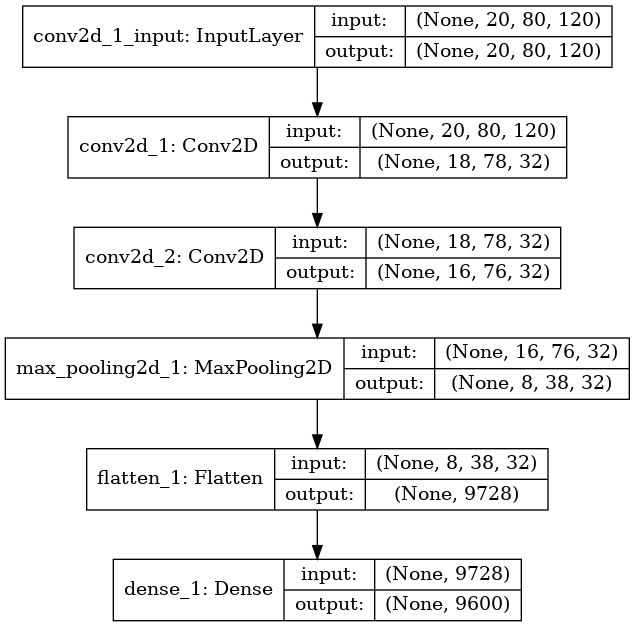
\includegraphics[width=0.8\textwidth]{ figures/net/NOREC_simple_raw.png}
			\caption{Estructura de \acrshort{cnn} para imágenes crudas.}
			\label{fig.cnn_raw}
		\end{center}
\end{figure}
\vspace{-10pt}

Una vez definida la red, se realizan experimentos con conjuntos de secuencias de imágenes crudas donde la complejidad de movimiento del píxel activo va aumentando de forma progresiva, tanto con el tipo de dinámica como en el número de grados de libertad para la misma dinámica.

\subsection{Influencia del número de muestras}
Con el objetivo de analizar la influencia que el número de muestras tiene en el aprendizaje de la red, se ha desarrollado un experimento en el que dicho número aumenta de forma progresiva, entrenando la estructura descrita anteriormente. Se han empleado muestras cuyos píxeles siguen una dinámica lineal de un único \acrshort{dof}, evaluando todas las redes con un mismo conjunto de \textit{test} de 1000 muestras. Los resultados se muestran en la gráfica de la Figura~\ref{fig.n_muestras}.

\begin{figure}[H]
		\begin{center}
			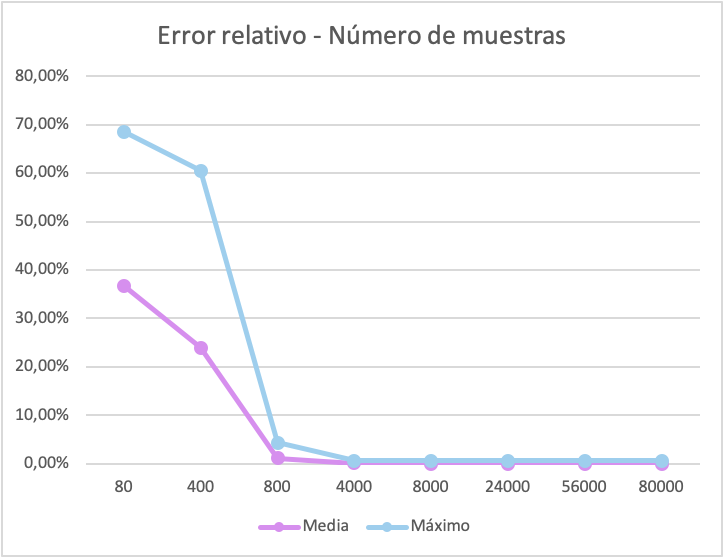
\includegraphics[width=0.7\textwidth]{ figures/test_raw/NOREC/n_muestras.png}
			\caption{Comparación del error relativo al aumentar el número de muestras de entrenamiento con \acrshort{cnn}~(Lineal, 1~\acrshort{dof}, 1000).}
			\label{fig.n_muestras}
		\end{center}
\end{figure}
\vspace{-10pt}


En el gráfico se puede comprobar cómo aumentar el número de muestras de entrenamiento produce un efecto positivo en las prestaciones de la red hasta un límite, a partir del cuál las prestaciones se mantienen. Este valor límite en el número de muestras dependerá de la complejidad de la dinámica  dinámica que rige el movimiento. Para las dinámicas más sencillas se necesitará un número menor de muestras de entrenamiento que para las más complejas. Mediante el el uso de un número adecuado de muestras en el entrenamiento se evita que no haya suficientes secuencias para que la red sea capaz de aprender y, por otro lado, que la red vea todos los ejemplos de la dinámica y memorice las relaciones entre la entrada y la salida, evitando la generalización.

\subsection{Predicción con dinámicas lineales}
Para abordar la predicción de fotogramas donde se representan objetos que siguen una dinámica lineal, se utiliza un \textit{dataset} compuesto por 10000 muestras. Este conjunto de datos se divide en tres, de tal forma que 8000 muestras se utilizan para el entrenamiento, 1000 para la validación y 1000 para el \textit{test}.\\

En la Figura~\ref{fig.raw_norec_lin_fix_10000} se muestran los resultados obtenidos al evaluar la \acrshort{cnn} propuesta entrenada con dicho conjunto cuando se considera un único \acrshort{dof}, la pendiente de la trayectoria del píxel activo. Se observa que las prestaciones de la red son buenas, pues se consigue un error relativo muy reducido en términos de media y máximo.

\begin{figure}[H]
		\begin{center}
			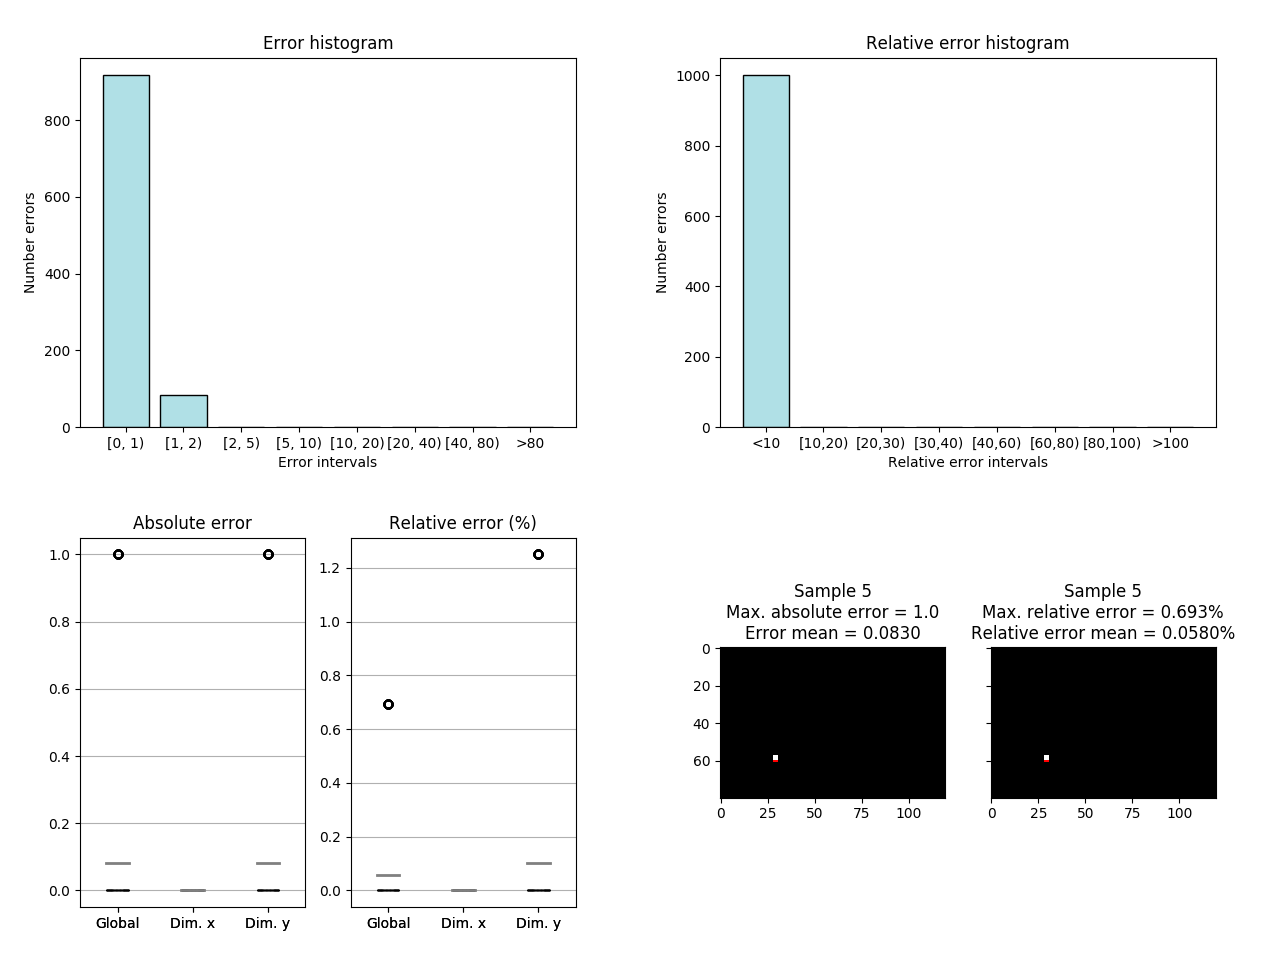
\includegraphics[width=0.8\textwidth]{ figures/test_raw/NOREC/linear_fix_10000.png}
			\caption{Resultados de \acrshort{cnn} con dinámica lineal de 1 \acrshort{dof}~(1000 muestras de \textit{test}).}
			\label{fig.raw_norec_lin_fix_10000}
		\end{center}
\end{figure}
\vspace{-10pt}


Al aumentar el grado de complejidad de la dinámica añadiendo un nuevo \acrshort{dof}, la posición vertical en la imagen desde la que el píxel activo comienza su movimiento recto. Los resultados obtenidos bajo esta nueva premisa, utilizando el mismo número de muestras y distribución de los subconjuntos que en el caso anterior, se muestran en la Figura~\ref{fig.raw_norec_lin_var_10000}.

\begin{figure}[H]
		\begin{center}
			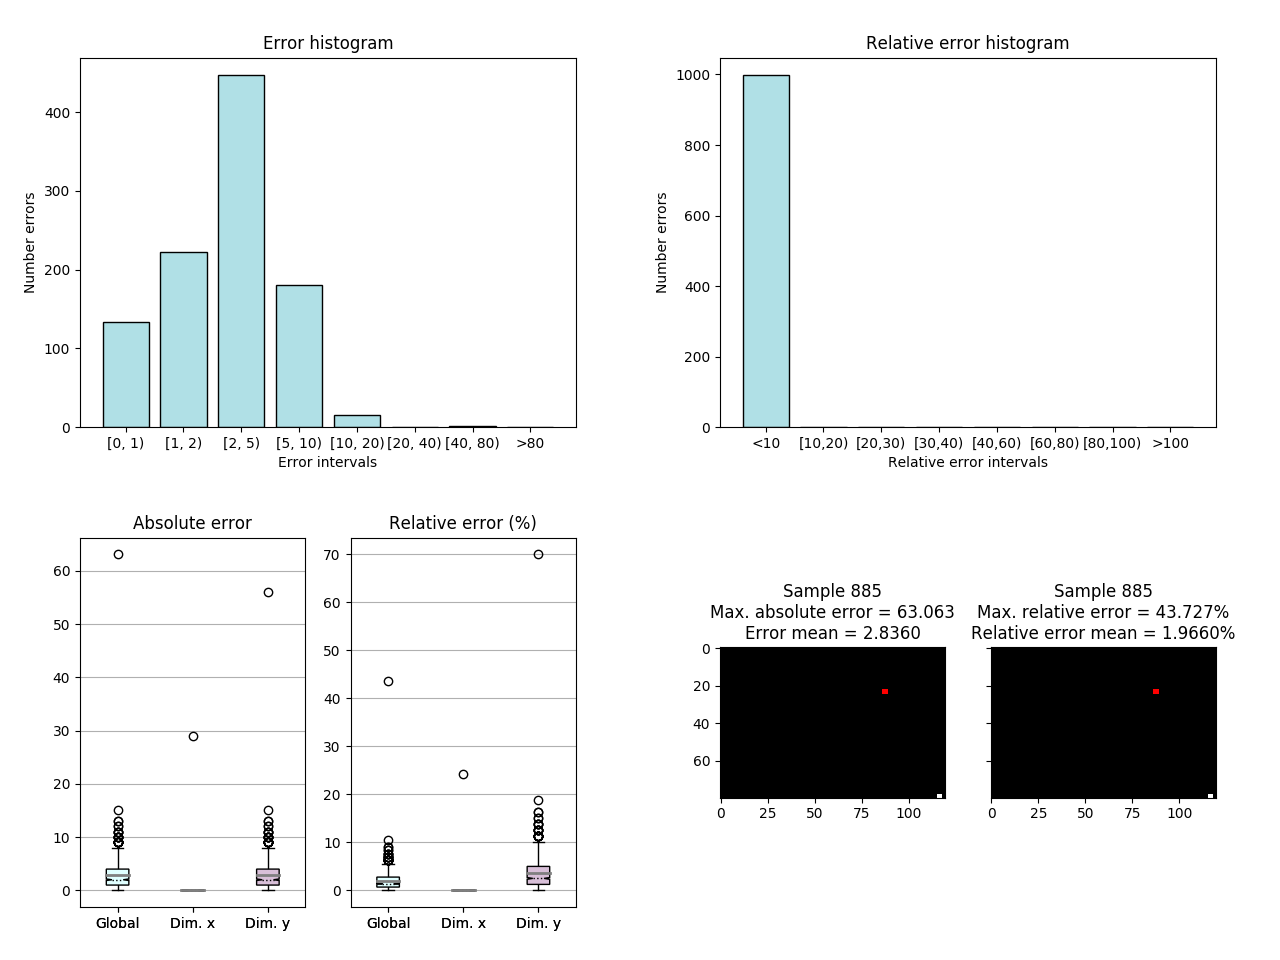
\includegraphics[width=0.8\textwidth]{ figures/test_raw/NOREC/linear_var_10000.png}
			\caption{Resultados de \acrshort{cnn} con dinámica lineal de 2 \acrshort{dof}~(1000 muestras de \textit{test}).}
			\label{fig.raw_norec_lin_var_10000}
		\end{center}
\end{figure}
\vspace{-10pt}

En esta ocasión, el resultado obtenido muestra un deterioro de las prestaciones de la red. Al tratar directamente con todos los píxeles de la imagen y no reducir la información a un par de valores (\textit{x}, \textit{y}), como en el caso de las modeladas, el número de parámetros que utiliza la red se ha elevado enormemente. Este hecho hace que, para el caso que se está tratando (dinámica lineal con 2\acrshort{dof}, la cantidad de ejemplos que se introducen a la red durante el entrenamiento pueda no ser suficiente. Para solucionar este problema  se decide aumentar el número de muestras del conjunto en un factor de 10, pasando de los 10000 ejemplos a 100000. La división en los tres subconjuntos se realiza con una asignación de 80000 para entrenamiento, 10000 para validación y 10000 para \textit{test}. Con este incremento en el número de muestras se vuelve a entrenar y a evaluar la misma estructura \acrshort{cnn}, obteniendo los resultados de la Figura~\ref{fig.raw_norec_lin_var_100000}.

\begin{figure}[H]
		\begin{center}
			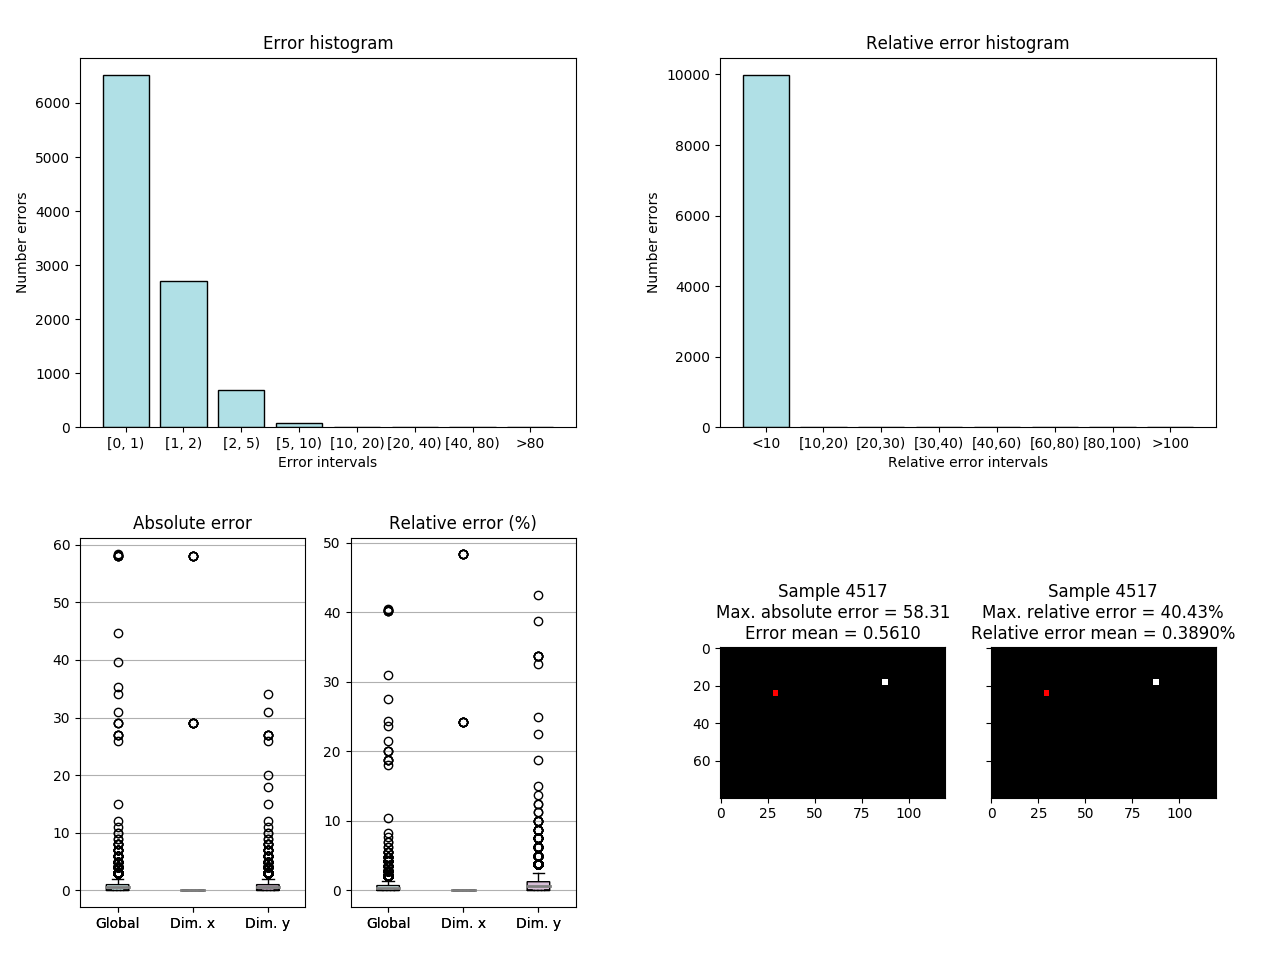
\includegraphics[width=0.8\textwidth]{ figures/test_raw/NOREC/linear_var_100000.png}
			\caption{Resultados de \acrshort{cnn} con dinámica lineal de 2 \acrshort{dof}~(10000 muestras de \textit{test}).}
			\label{fig.raw_norec_lin_var_100000}
		\end{center}
\end{figure}
\vspace{-10pt}

Se observa que con el aumento en el número de muestras de entrenamiento se mejoran las prestaciones de la red en términos de promedio del error relativo, pero siguen existiendo algunos \textit{outliers}, valores atípicos que perjudican a la predicción y no permiten obtener resultados óptimos.

\subsection{Predicción con dinámicas parabólicas}
Para abordar la predicción de fotogramas donde se representan objetos que siguen una dinámica parabólica se utiliza un \textit{dataset} compuesto por 100000 muestras. Este conjunto de datos queda dividido en tres subconjuntos, utilizando 80000 muestras para el entrenamiento, 10000 para la validación y 10000 para el \textit{test}.\\

Se comienza el estudio con el caso más sencillo de la dinámica, un único \acrshort{dof}~(valor de \textit{a}). Los resultados obtenidos se reflejan en la Figura~\ref{fig.raw_norec_par_fix_100000}. Las prestaciones de la red son muy buenas, se obtienen valores muy bajos de error y el número de \textit{outliers} es también muy reducido.

\begin{figure}[H]
		\begin{center}
			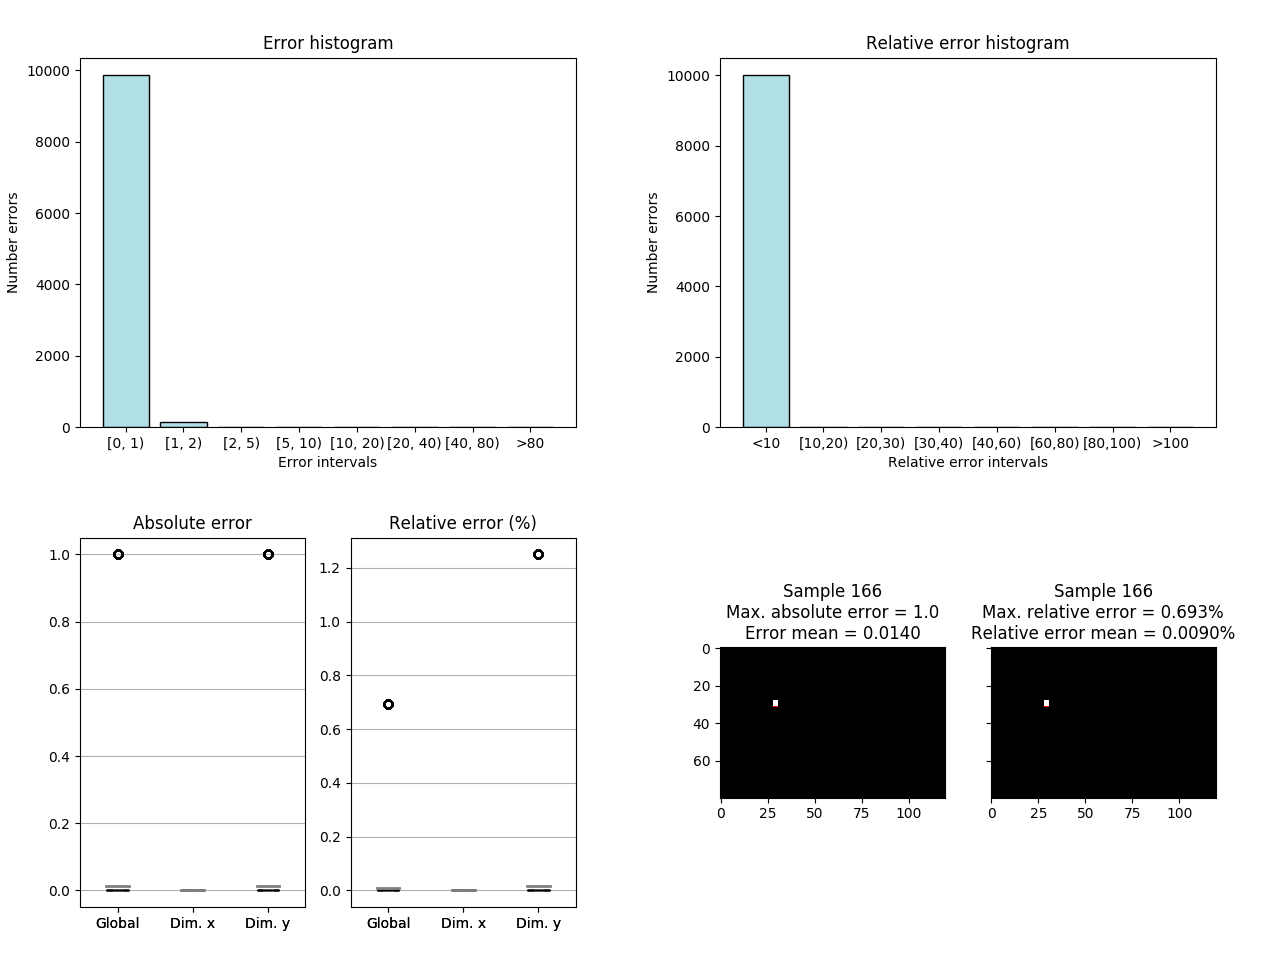
\includegraphics[width=0.8\textwidth]{ figures/test_raw/NOREC/parabolic_fix_100000.png}
			\caption{Resultados de \acrshort{cnn} con dinámica parabólica de 1 \acrshort{dof}~(10000 muestras de \textit{test}).}
			\label{fig.raw_norec_par_fix_100000}
		\end{center}
\end{figure}
\vspace{-10pt}

Se aumenta la complejidad de la dinámica con un nuevo \acrshort{dof}, la posición vertical inicial del píxel en la imagen (valor de \textit{c}), manteniendo el número de muestras y la distribución de los subconjuntos  del caso anterior. Los resultados obtenidos sobre la red entrenada con este conjunto se muestran en la Figura~\ref{fig.raw_norec_par_var_100000}. En esta ocasión, al contrario que ocurría en la dinámica lineal, el aumento de la complejidad, aunque empeora los resultados, no provoca que la red pierda su capacidad predictiva.\\

Finalmente, dentro de esta dinámica se establecen 3 \acrshort{dof}. Se utiliza el mismo número de muestras por subconjunto que en los casos anteriores, obteniendo los resultados de la Figura~\ref{fig.raw_norec_par_var1_100000}. En ella se refleja que los valores de error son elevados, se produce un gran número de \textit{outliers} y la caja de los \textit{boxplot} se separa ligeramente del valor nulo. Con todo esto, las prestaciones de la red se reducen respecto a los casos anteriores, empeorando la capacidad predictiva de la red.

\begin{figure}[H]
		\begin{center}
			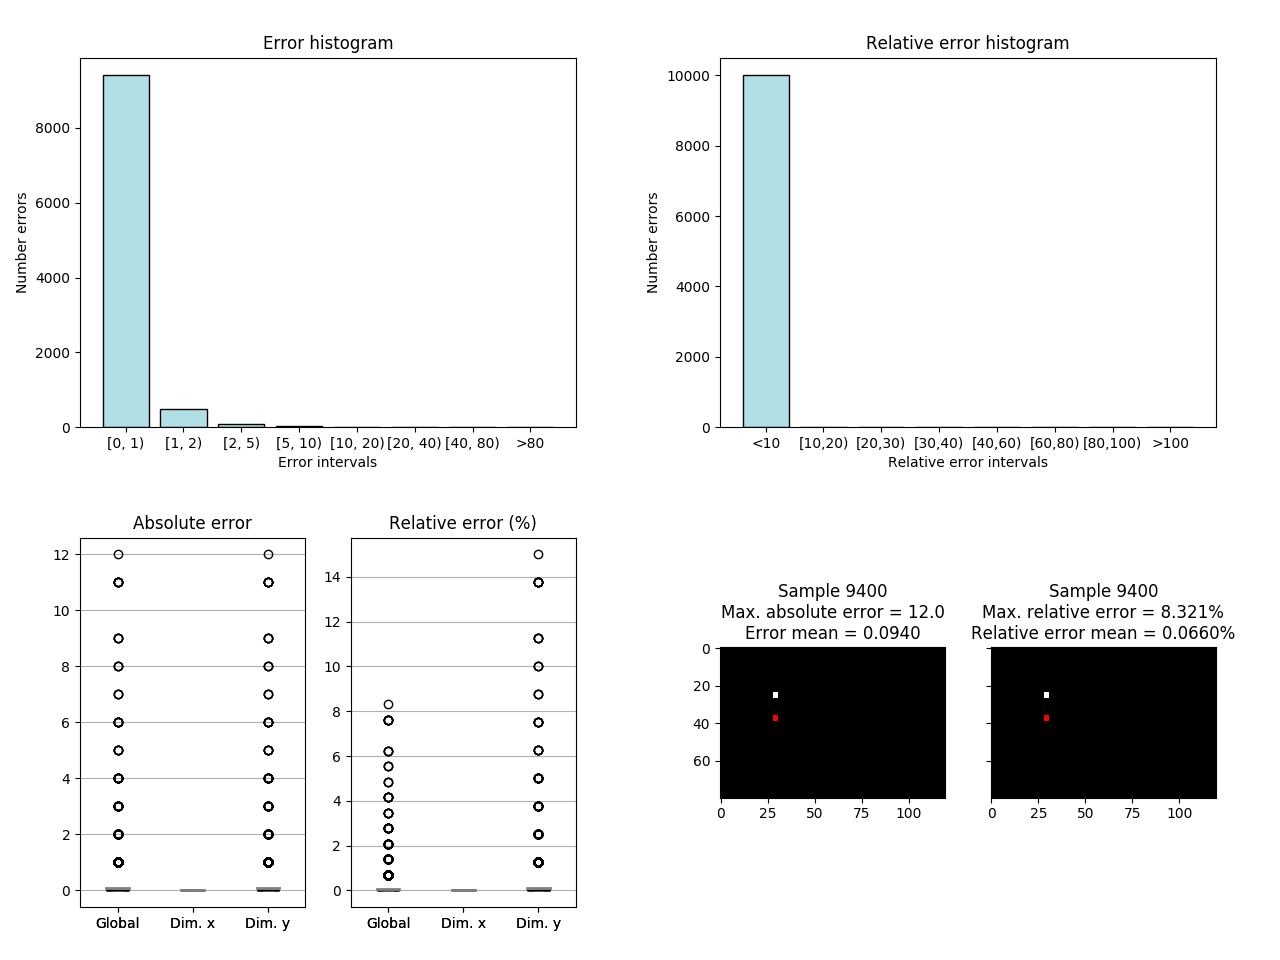
\includegraphics[width=0.8\textwidth]{ figures/test_raw/NOREC/parabolic_var_100000.png}
			\caption{Resultados de \acrshort{cnn} con dinámica parabólica de 2 \acrshort{dof}~(10000 muestras de \textit{test}).}
			\label{fig.raw_norec_par_var_100000}
		\end{center}
\end{figure}
\vspace{-30pt}
\begin{figure}[H]
		\begin{center}
			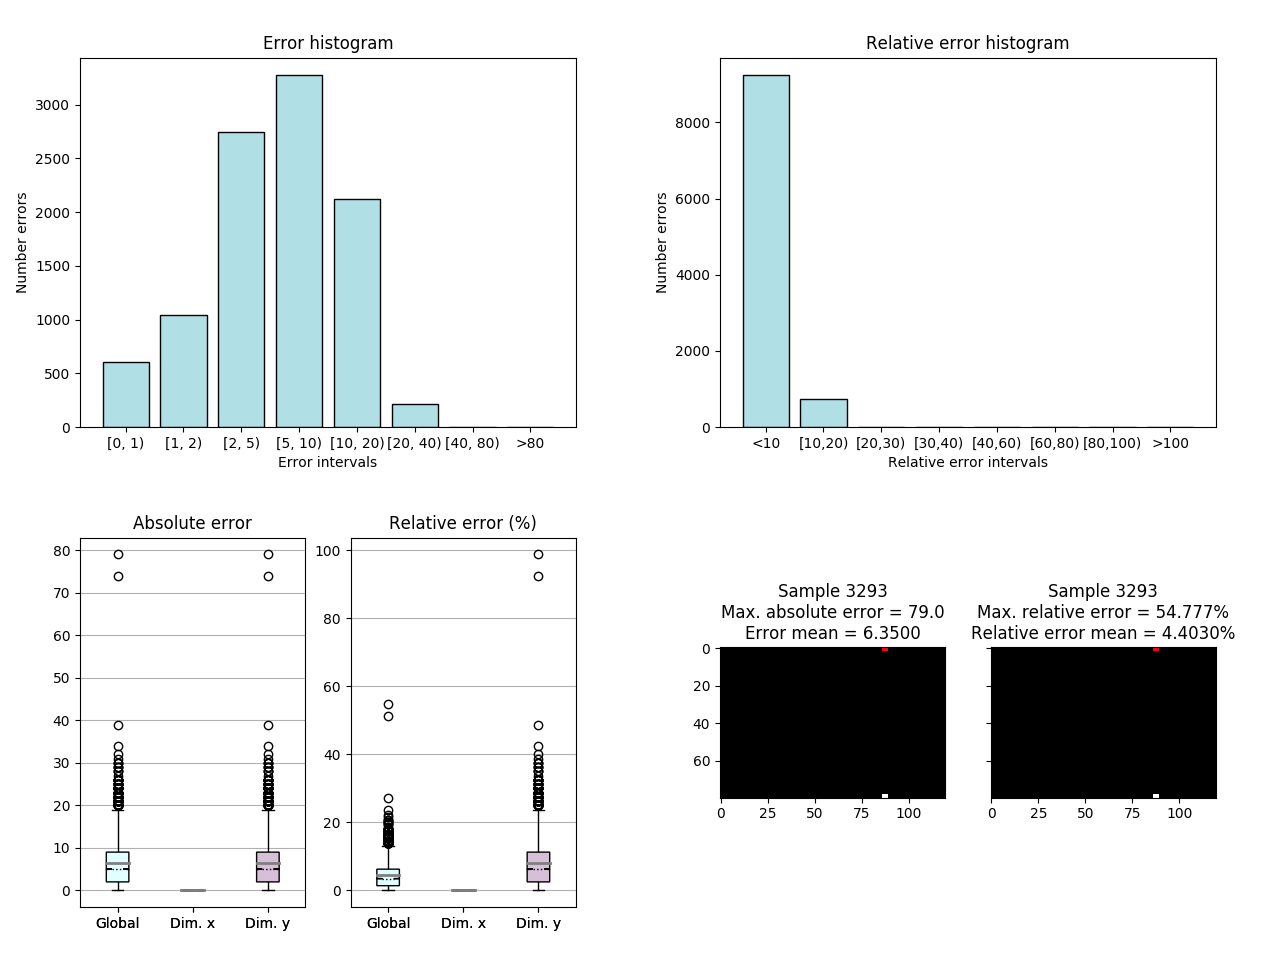
\includegraphics[width=0.8\textwidth]{ figures/test_raw/NOREC/parabolic_var1_100000.png}
			\caption{Resultados de \acrshort{cnn} con dinámica parabólica de 3 \acrshort{dof}~(10000 muestras de \textit{test}).}
			\label{fig.raw_norec_par_var1_100000}
		\end{center}
\end{figure}
\vspace{-10pt}

\subsection{Predicción con dinámicas sinusoidales}
Para abordar la predicción de fotogramas que representan objetos que siguen una dinámica sinusoidal, se utiliza un \textit{dataset} compuesto por 100000 muestras. Sobre el total de muestras establecido se realiza una división de tal forma que 80000 muestras se utilizan para el entrenamiento, 10000 para la validación y 10000 para el \textit{test}.\\

Se comienza con la variante más sencilla de esta dinámica, que deja como parámetro aleatorio la frecuencia de la sinusoide, 1~\acrshort{dof}. En la Figura~\ref{fig.raw_norec_sin_fix_100000} se muestran los resultados obtenidos, donde se puede comprobar que la red tiene muy buenas prestaciones para este caso.
\begin{figure}[H]
		\begin{center}
			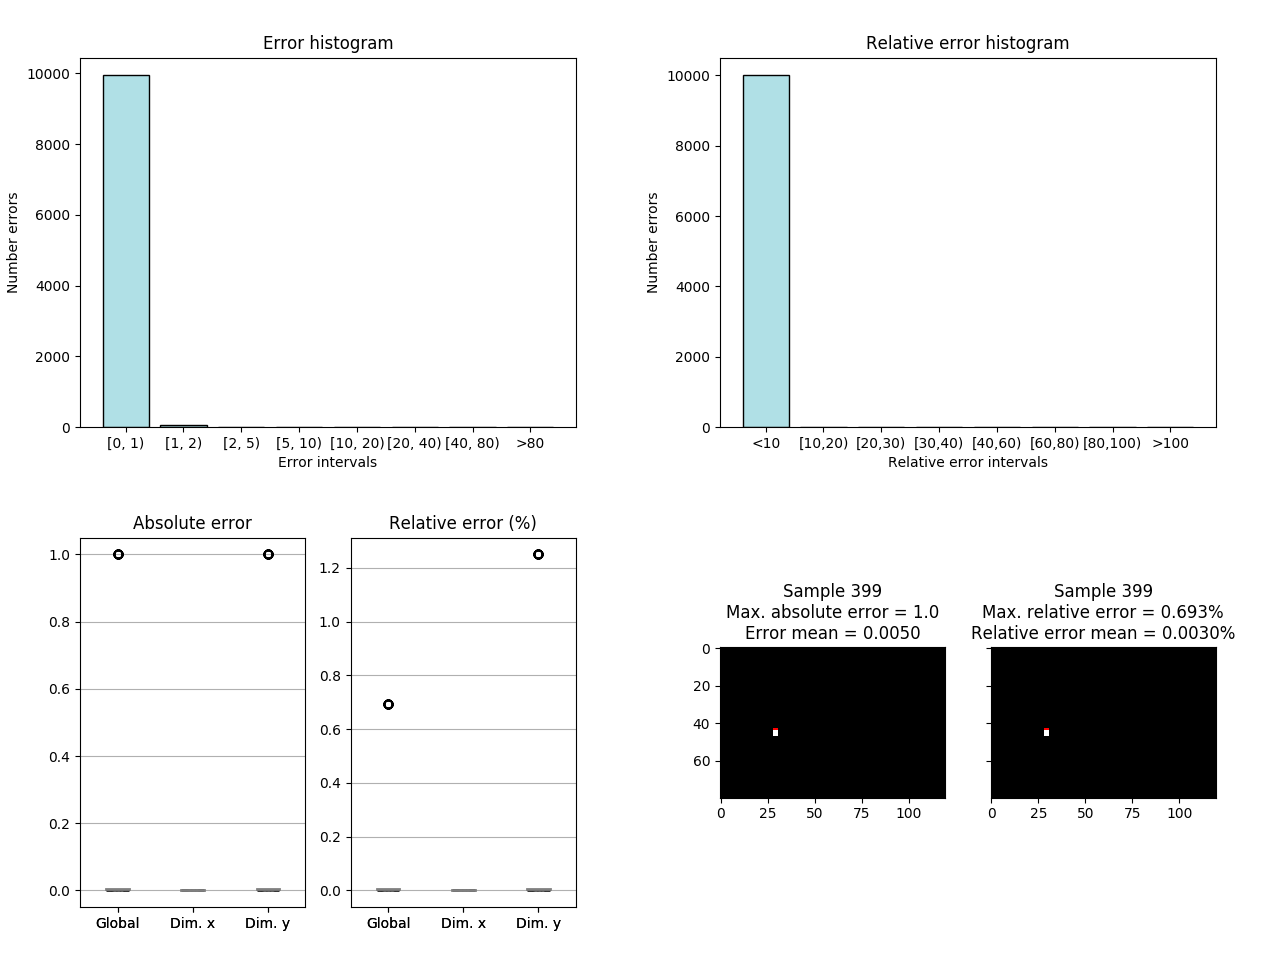
\includegraphics[width=0.8\textwidth]{ figures/test_raw/NOREC/sin_fix_100000.png}
			\caption{Resultados de \acrshort{cnn} con dinámica sinusoidal de 1 \acrshort{dof}~(10000 muestras de \textit{test}).}
			\label{fig.raw_norec_sin_fix_100000}
		\end{center}
\end{figure}
\vspace{-10pt}

A continuación, se permite que la posición vertical inicial del píxel en la imagen tome también un valor aleatorio, estableciendo la dinámica con 2~\acrshort{dof}. Tras entrenar y evaluar la red propuesta con los subconjuntos correspondientes, cuyas características son las mismas que en casos anteriores, se obtienen los resultados de la Figura~\ref{fig.raw_norec_sin_var_100000}. Estos valores reflejan un deterioro de las prestaciones de la red por la complejidad de la dinámica. Los valores de error han aumentado considerablemente, especialmente el máximo, y se obtiene un número de \textit{outliers} mucho mayor que en el caso más sencillo. Con estos resultados, se establece el límite de predicción con la \acrshort{cnn} propuesta para dinámicas sinusoidales en un único \acrshort{dof}.

\begin{figure}[H]
		\begin{center}
			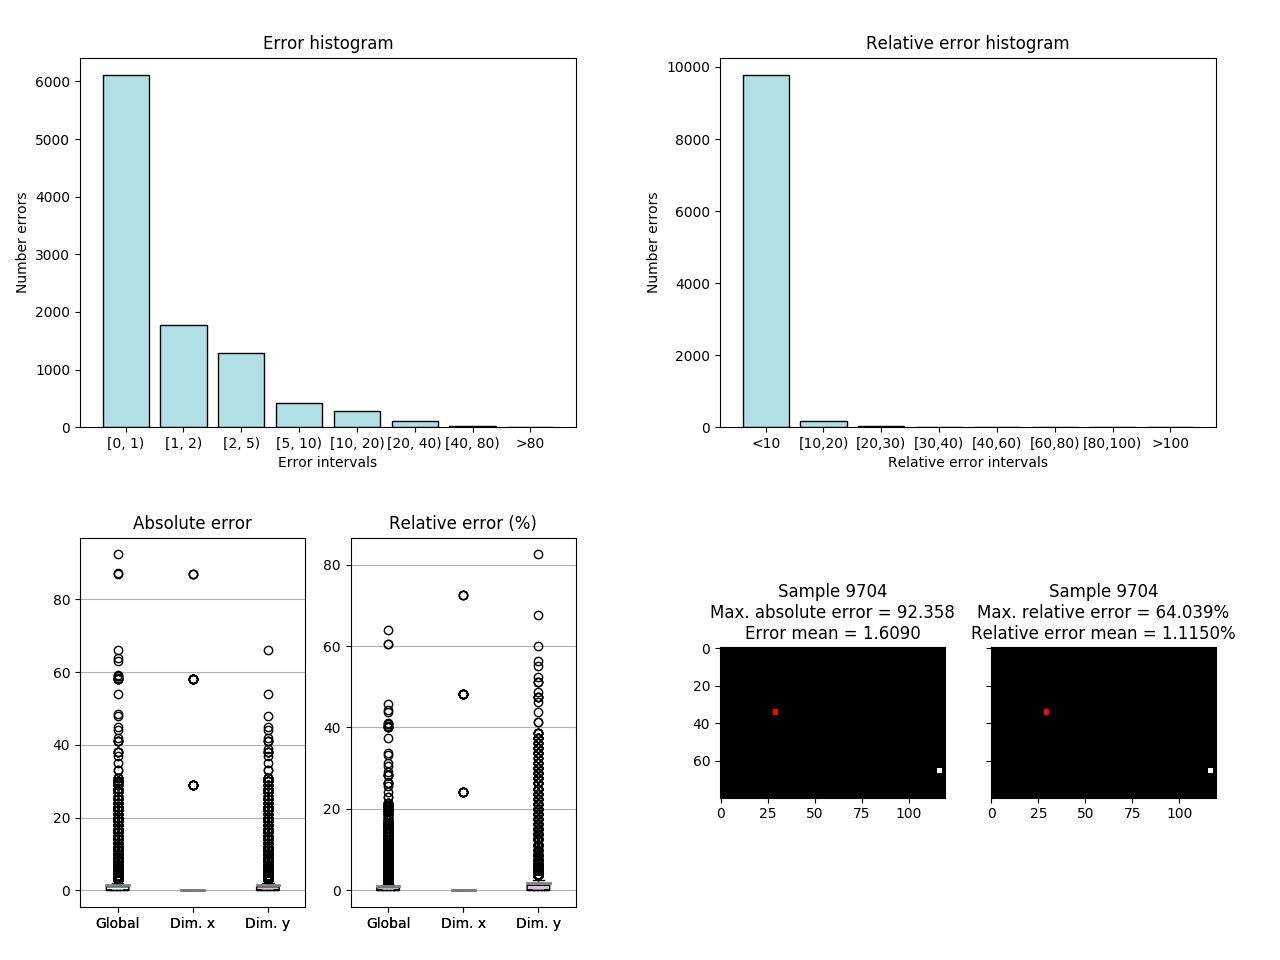
\includegraphics[width=0.8\textwidth]{ figures/test_raw/NOREC/sin_var_100000.png}
			\caption{Resultados de \acrshort{cnn} con dinámica sinusoidal de 2 \acrshort{dof}~(10000 muestras de \textit{test}).}
			\label{fig.raw_norec_sin_var_100000}
		\end{center}
\end{figure}
\vspace{-10pt}

\subsection{Resumen de resultados}

En la Tabla~\ref{tab.cnn} se muestra un resumen de los resultados alcanzados en cada dinámica con imágenes de píxeles 2D. Para la interpretación de esta tabla se ha establecido un código de cuatro colores que reflejan, de mejor a peor, los resultados obtenidos en cada experimento. La secuencia de colores utilizada comienza con el verde oscuro para resultados muy buenos, pasando por el verde claro y el naranja, para terminar con el rojo, que indica malos resultados. Para  realizar una comparación equitativa, se ha vuelto a evaluar la dinámica lineal de 1~\acrshort{dof} con 10000, proporcionando un promedio de error relativo de 0.07\%. 

\begin{table}[H]
	\centering
	\begin{tabular}{{|l|c|c|}}
		\hline
		\multicolumn{2}{|c|}{\textbf{Dinámica}} & \textbf{\acrshort{cnn}}\\ \hline 
		\multirow{2}{*}{Lineal}
		&1~\acrshort{dof} & \cellcolor{darkgreen}{0.07\%}\\
		\cline{2-3}
        &2~\acrshort{dof} & \cellcolor{greenyellow}{0.39\%}\\
        \hline
        \multirow{3}{*}{Parabólica}
        &1~\acrshort{dof} & \cellcolor{darkgreen}0.01\%\\
        \cline{2-3}
        &2~\acrshort{dof} & \cellcolor{darkgreen}0.07\%\\
        \cline{2-3}
        &3~\acrshort{dof} & \cellcolor{red}4.40\%\\ 
        \hline
        \multirow{2}{*}{Sinusoidal}
        &1~\acrshort{dof} & \cellcolor{darkgreen}0.003\%\\
        \cline{2-3}
        &2~\acrshort{dof} & \cellcolor{myorange}1.12\%\\
        \hline
	\end{tabular}
	\caption{Promedio del error relativo en \textit{test} al evaluar la \acrshort{cnn} con imágenes modeladas y distintas dinámicas (10000 muestras de \textit{test}).}
	\label{tab.cnn}
\end{table}

\section{Arquitectura recurrente: Convolucional + LSTM}
Una vía de investigación en cuanto al efecto de introducir la recurrencia en la predicción de imágenes es combinar una capa convolucional, que capte las relaciones espaciales, con una capa \acrshort{lstm} posterior, para las relaciones temporales. La estructura propuesta se muestra en la Figura~\ref{fig.cnn_lstm_raw}.

\begin{figure}[H]
		\begin{center}
			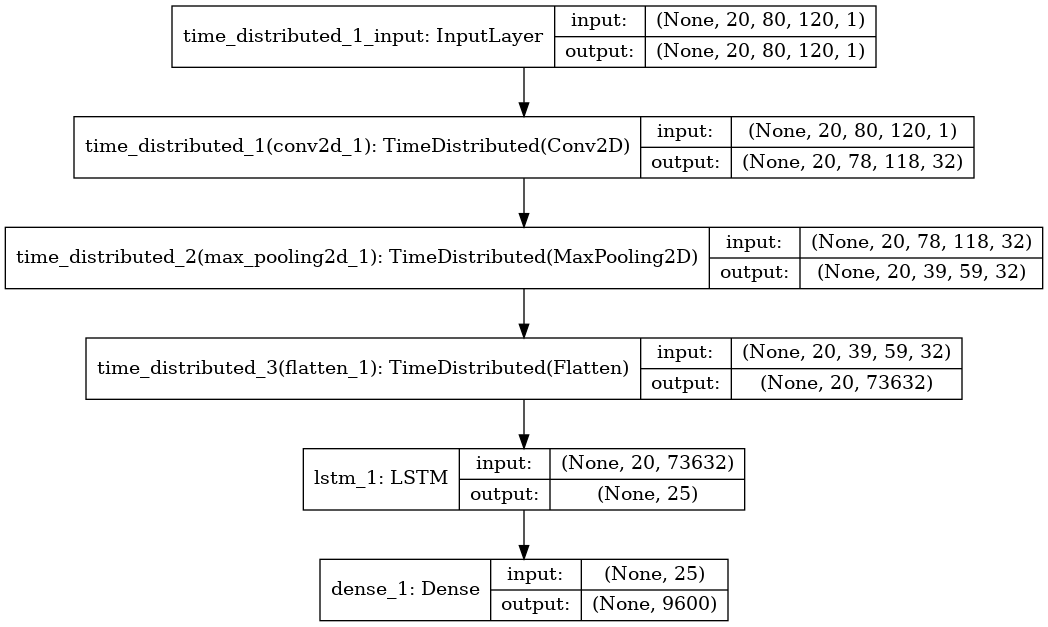
\includegraphics[width=0.9\textwidth]{ figures/net/REC_simple_raw.png}
			\caption{Estructura de \acrshort{cnn}+\acrshort{lstm} para imágenes crudas.}
			\label{fig.cnn_lstm_raw}
		\end{center}
\end{figure}
\vspace{-10pt}

La red consta de una capa convolucional de 32 neuronas seguida de su correspondiente capa de reducción. Tras la estructura propia de las \acrshort{cnn} se añade una capa para \textit{flatten} para obtener un vector de una dimensión que será la entrada a la única capa \acrshort{lstm} con 25 neuronas.

\subsection{Predicción con dinámicas lineales}
Para estudiar el efecto de la recurrencia con la arquitectura de red propuesta, se comienza con el caso más sencillo de todos: dinámica lineal de pendiente nula y con posición vertical inicial del píxel fija. El conjunto consta de  1000 muestras, de las cuales 800 son para entrenamiento, 100 para validación y otras 100 para \textit{test}. Al evaluar la red \acrshort{cnn} propuesta en la Sección~\ref{sec.raw_norec_cnn} con el mismo conjunto se obtiene un error completamente nulo, según se muestra en la Figura~\ref{fig.raw_norec_urm_fix_1000}; sin embargo, al introducir la capa \acrshort{lstm}, la red pierde toda su capacidad predictiva pasando de un 100\% de acierto a un 70\%, según se muestra en la Figura~\ref{fig.raw_rec_urm_fix_1000}.

\begin{figure}[H]
		\begin{center}
			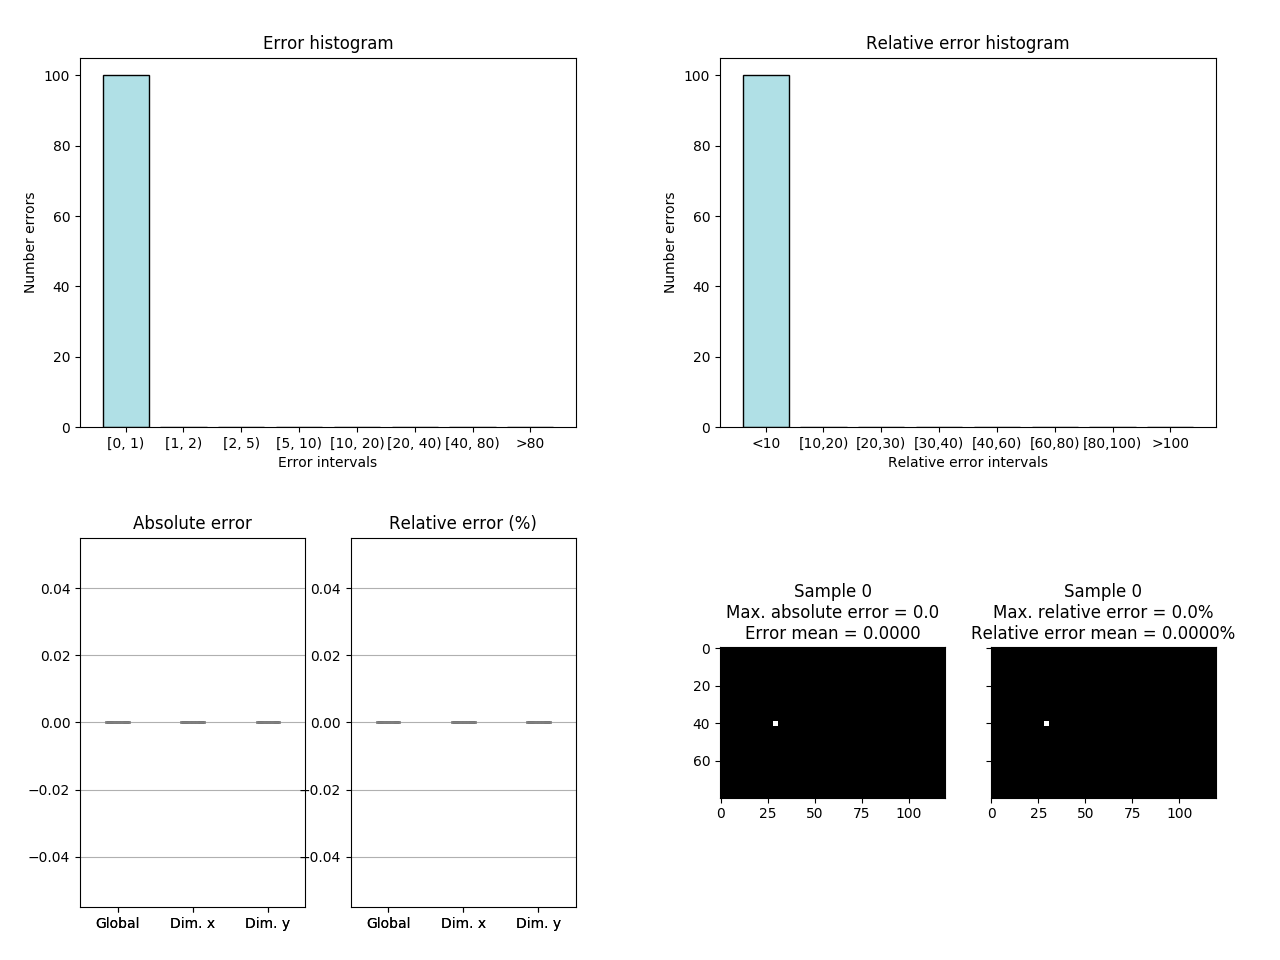
\includegraphics[width=0.8\textwidth]{ figures/test_raw/NOREC/URM_fix_1000.png}
			\caption{Resultados de \acrshort{cnn} con dinámica lineal, pendiente nula y altura fija~(100 muestras de \textit{test}).} 
			\label{fig.raw_norec_urm_fix_1000}
		\end{center}
\end{figure}
\vspace{-10pt}

\begin{figure}[H]
		\begin{center}
			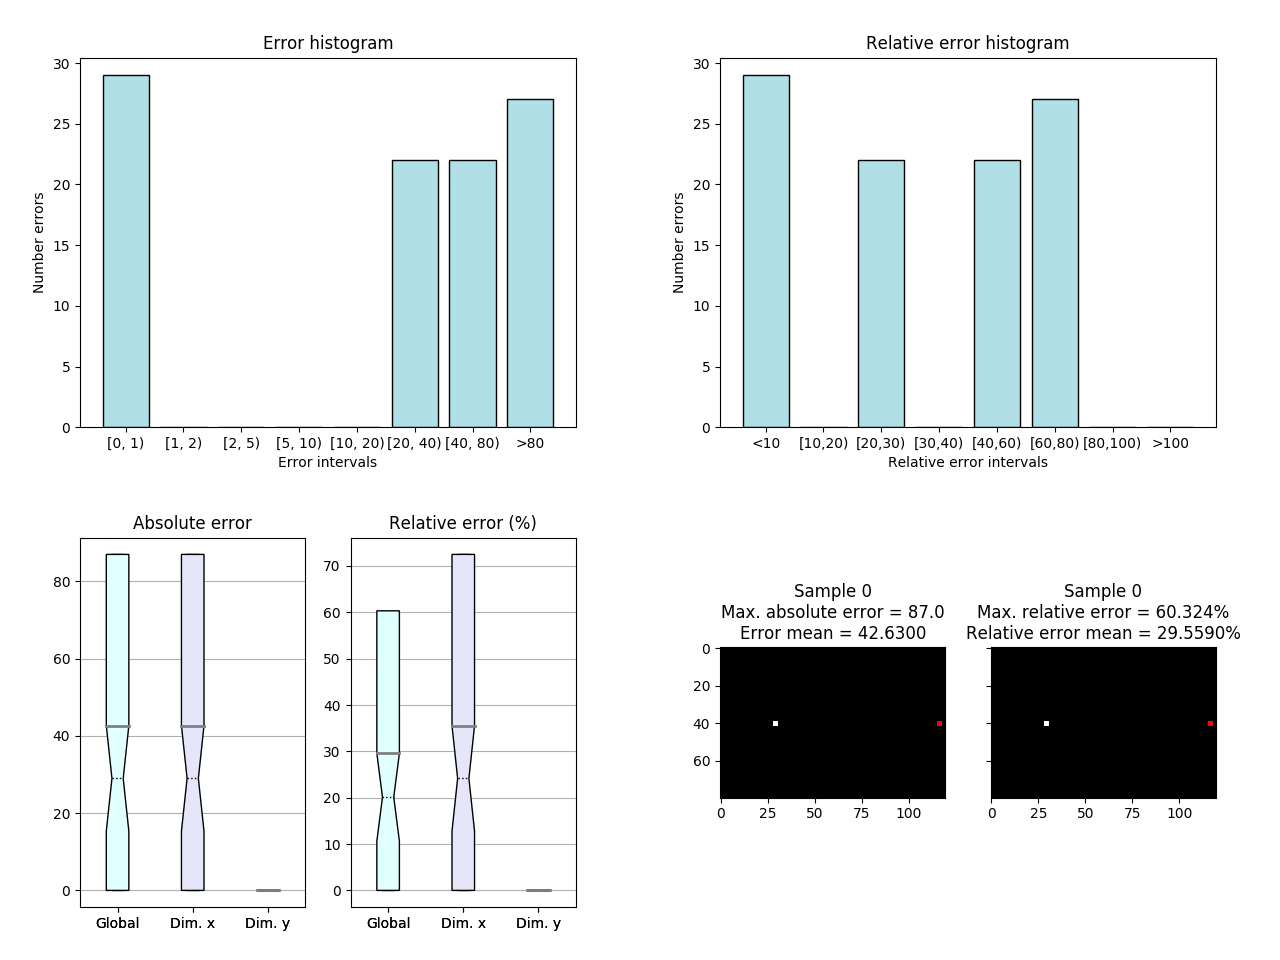
\includegraphics[width=0.8\textwidth]{ figures/test_raw/REC/CONV+LSTM/URM_fix_1000.png}
			\caption{Resultados de \acrshort{cnn}+\acrshort{lstm} con dinámica lineal, pendiente nula y altura fija~(100 muestras de \textit{test}).} 
			\label{fig.raw_rec_urm_fix_1000}
		\end{center}
\end{figure}
\vspace{-10pt}

Con estos resultados se puede concluir que analizar las relaciones temporales de forma independiente a las espaciales no parece una buena estrategia.

\subsection{Extensión gradual del punto activo}
Una de las posibles causas de que esta estrategia de combinar una \acrshort{cnn} con una \acrshort{lstm} no funcione correctamente es que se están empleando  imágenes con un único píxel activo, complicando a la red la tarea de encontrar correlaciones espaciales. Para analizar este hecho se decide ampliar la zona activa de la imagen, reduciendo de forma gradual el nivel de intensidad de los píxeles alrededor del píxel activo, haciendo uso de una función gaussiana isotrópica. En la Figura~\ref{fig.pixel} se muestra tanto el píxel utilizado hasta ahora, que denominaremos píxel discreto, como el resultado de convolucionar un filtro gaussiano con centro en dicho píxel y entorno activo 5x5.

\begin{figure}[H]
		\begin{center}
			\subfigure[]{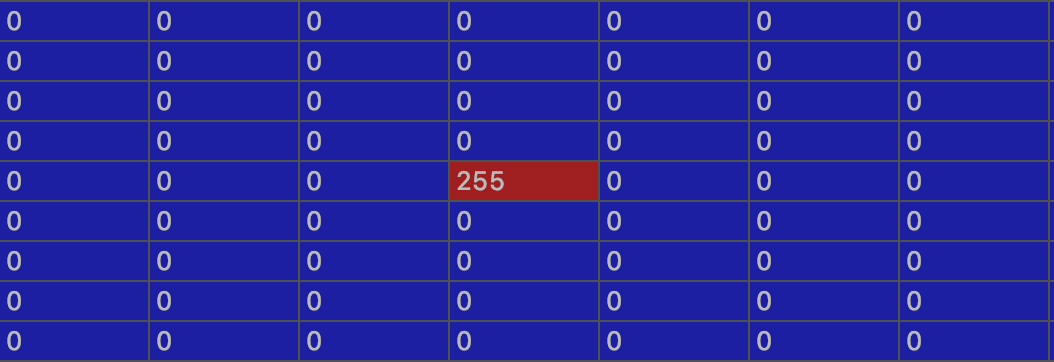
\includegraphics[width=0.5\textwidth]{ figures/pixel_discreto.png}}
	        \subfigure[]{\frame{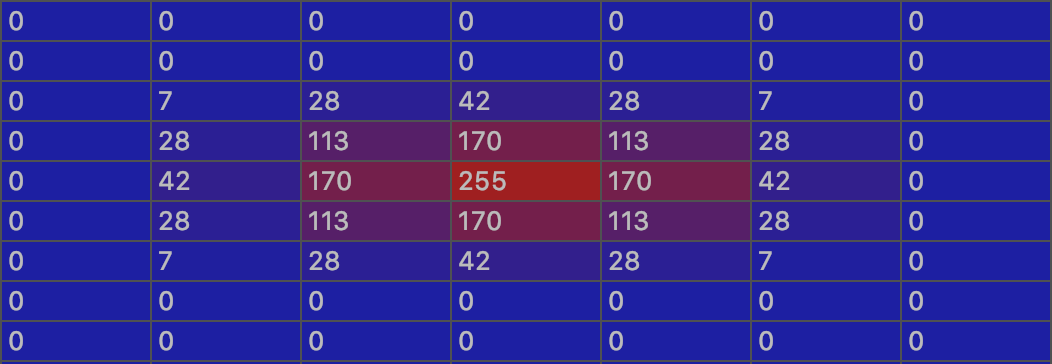
\includegraphics[width=0.5\textwidth]{ figures/pixel_gaussiano.png}}}
	        \caption{Ejemplos de píxel: (a)~Discreto y (b)~Expandido.}
			\label{fig.pixel}
		\end{center}
\end{figure}
\vspace{-10pt}

La intuición subyacente es que, al extender el píxel, los algoritmos que hacen uso de correlación espacial pueden tener valores gradualmente crecientes al acercarse a una correlación máxima, y tal vez durante el aprendizaje se vean ayudados a converger hacia ese máximo. Con un píxel discreto las correlaciones entre los píxeles de la imagen son todas nulas excepto en el máximo, lo que no ayuda a los algoritmos de aprendizaje (que se suelen apoyar en gradientes) a encontrarlo: en las cercanías del píxel activo las correlaciones valen igual que si se está lejos del mismo.\\

Para analizar la repercusión que tiene en evaluación el aprendizaje con extensión del píxel, se emplea el mismo conjunto de dinámica lineal utilizado anteriormente, aplicándole a las imágenes una convolución con el filtro gaussiano antes de su entrada a la red. En la Figura~\ref{fig.raw_rec_urm_fix_1000_gauss} se muestran los resultados de este nuevo experimento.

\begin{figure}[H]
		\begin{center}
			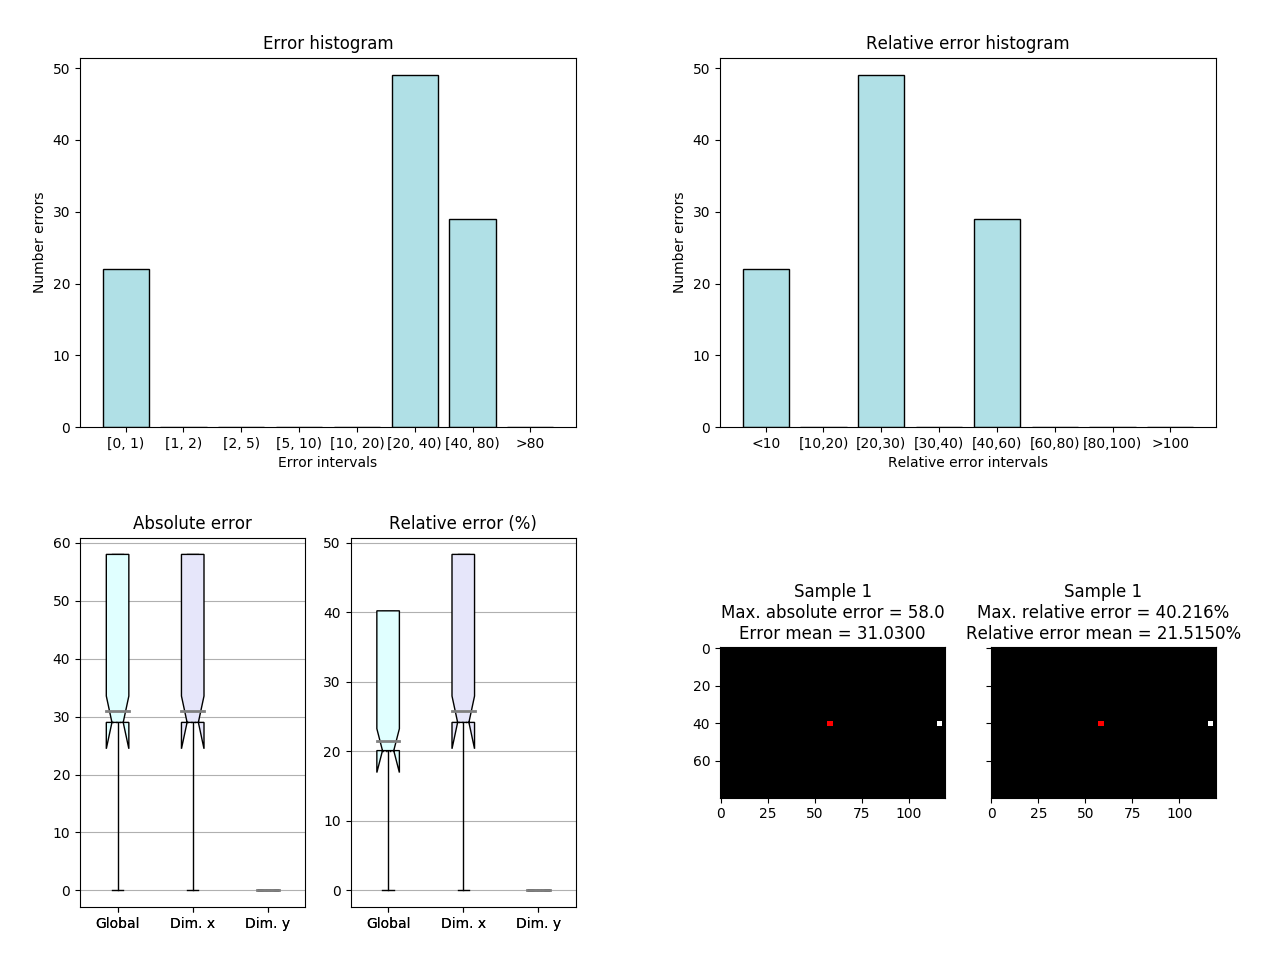
\includegraphics[width=0.8\textwidth]{ figures/test_raw/REC/CONV+LSTM/URM_fix_1000_Gauss.png}
			\caption{Resultados de \acrshort{cnn}+\acrshort{lstm} con píxel extendido en dinámica lineal, pendiente nula y altura fija~(100 muestras de \textit{test}).} 
			\label{fig.raw_rec_urm_fix_1000_gauss}
		\end{center}
\end{figure}
\vspace{-10pt}

Aunque los resultados han mejorado en términos de valores medios, la red continúa sin ser capaz de predecir correctamente. Además, la caja del \textit{boxplot} se ha visto desplazada hacia arriba, dejando los valores más bajos de error como \textit{outliers} de los resultados. Con este análisis se concluye que, por un lado, la estrategia de combinar por separado ambas relaciones no es adecuada, y por el otro, extender el píxel para facilitar el análisis de las correlaciones espaciales en la imagen no es una mejora.

\subsection{Resumen de resultados}
A modo de resumen, la Tabla~\ref{tab.conv+lstm} se muestran los resultados de los experimentos relacionados con la estructura que combina una capa convolucional con una \acrshort{lstm} posterior a modo de resumen.

\begin{table}[H]
	\centering
	\begin{tabular}{{|l|c|c|c|}}
		\hline
		\multicolumn{2}{|c|}{\textbf{Dinámica}} & \textbf{\acrshort{cnn}} & \textbf{\acrshort{cnn}+\acrshort{lstm}}\\ \hline 
		\multirow{2}{*}{Lineal}
		&Discreto & \cellcolor{darkgreen}{0.0\%} & \cellcolor{red}{29.6\%}\\
		\cline{2-3}
        &Gaussiano & \cellcolor{gray!30} & \cellcolor{red}{21.5\%}\\
        \hline
	\end{tabular}
	\caption{Promedio del error relativo en \textit{test} al evaluar la red \acrshort{cnn}+\acrshort{lstm} con imágenes modeladas y distintas dinámicas (10000 muestras de \textit{test}).}
	\label{tab.conv+lstm}
\end{table}

\section{Arquitectura recurrente: ConvLSTM-1}
Otra vía a explorar, en cuanto al efecto de la recurrencia en la capacidad de predicción de las redes, es el uso de las redes \textit{ConvLSTM} presentadas en el Apartado~\ref{ap.convLSTM}. Para ello, se define la estructura de red de la Figura~\ref{fig.convLSTM1}.

\begin{figure}[H]
		\begin{center}
			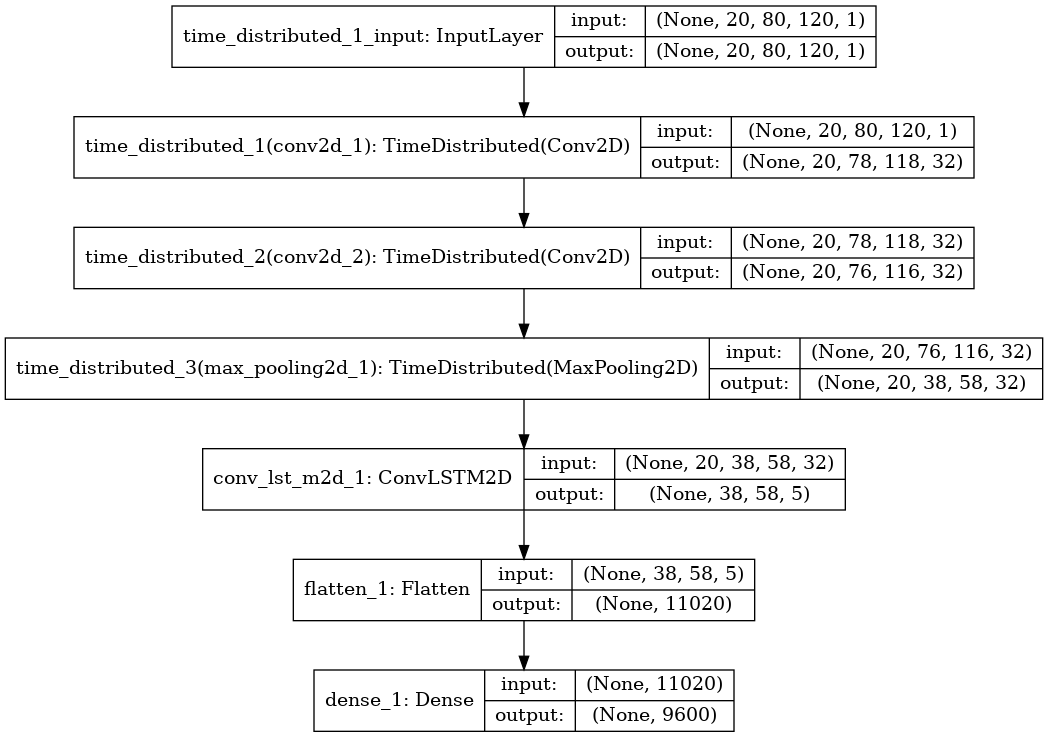
\includegraphics[width=0.9\textwidth]{ figures/net/REC_convLSTM_simple.png}
			\caption{Estructura de ConvLSTM-1 para imágenes crudas.}
			\label{fig.convLSTM1}
		\end{center}
\end{figure}
\vspace{-10pt}

Debido a la cantidad de valores en cada una de las secuencias de entrada, 20 imágenes con $80 \times 120$ píxeles, es necesario realizar una reducción de la dimensionalidad para que la máquina sea capaz de procesar todos los valores. Para ello se introduce tras la entrada de la red dos capas convolucionales, de 32 neuronas cada una, seguidas de su capa de \textit{pooling}, que reducen la cantidad de valores a procesar. Posteriormente, se utiliza una única capa \textit{ConvLSTM} de 5 neuronas que será la encargada de analizar las correlaciones espacio-temporales de las entradas.\\

Con la estructura de red definida se realizan experimentos sobre todas las dinámicas propuestas, aumentando de forma progresiva la complejidad de cada una de ellas.

\subsection{Predicción con dinámicas lineales}
Para la predicción en imágenes cuyo píxel se mueve siguiendo una dinámica lineal con un solo \acrshort{dof}, se utiliza el mismo conjunto que en el caso no recurrente: un total del 10000 muestras repartidas en 8000 para entrenar, 1000 para validar y 1000 para evaluar. La Figura~\ref{fig.raw_convlstm1_lin_fix_10000} muestra los resultado obtenidos con dicho conjunto.

\begin{figure}[H]
		\begin{center}
			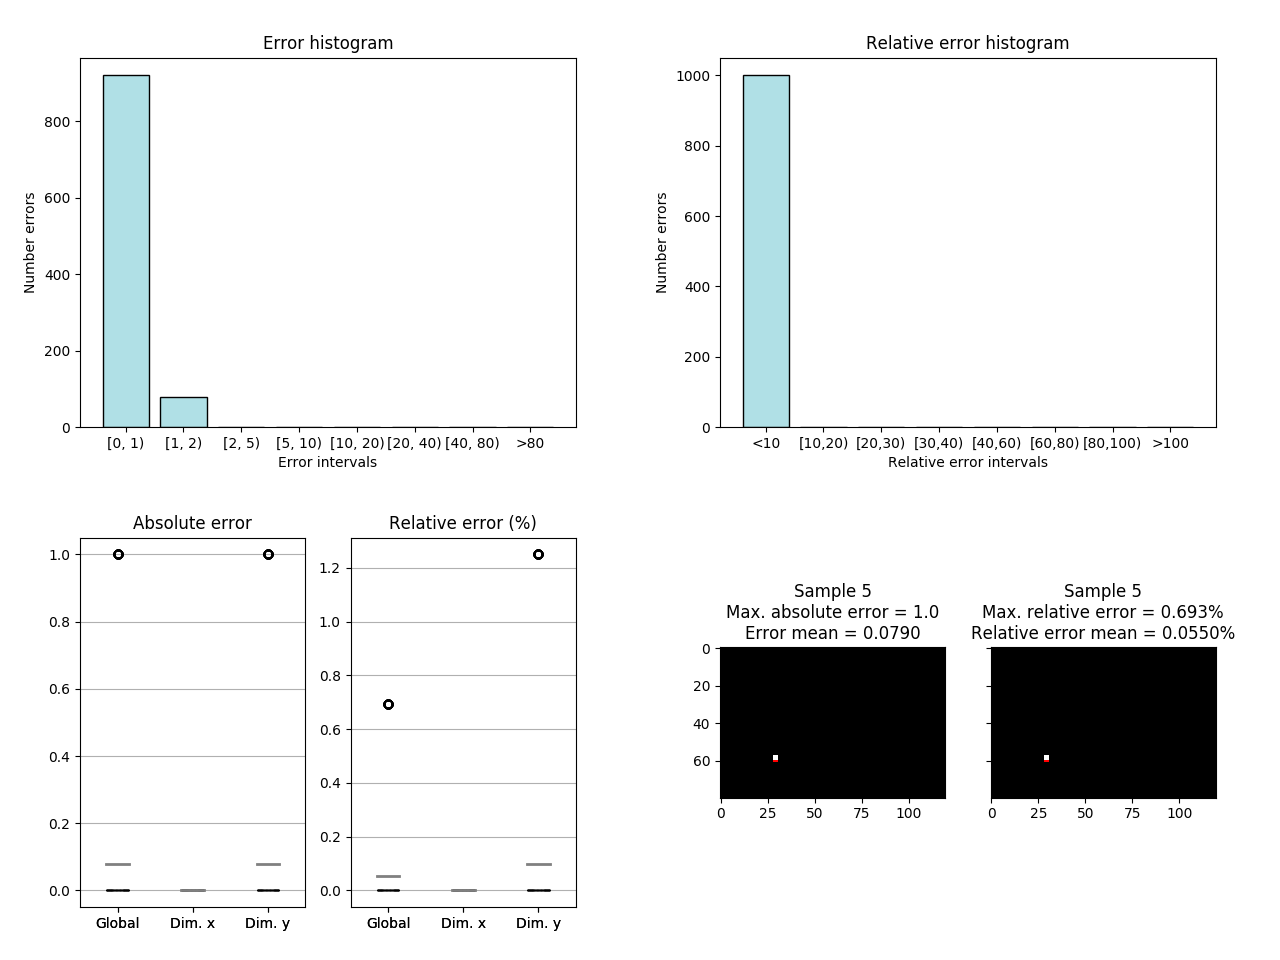
\includegraphics[width=0.8\textwidth]{ figures/test_raw/REC/ConvLSTM_simple/linear_fix_10000.png}
			\caption{Resultados de ConvLSTM-1 con dinámica lineal de 1 \acrshort{dof}~(1000 muestras de \textit{test}).}
			\label{fig.raw_convlstm1_lin_fix_10000}
		\end{center}
\end{figure}
\vspace{-10pt}

Los resultados obtenidos para esta dinámica con un \acrshort{dof} son similares a los del caso no recurrente, proporcionando una muy buena capacidad predictiva para ambos tipos de redes. Estos resultados indican que la nueva estructura de red recurrente no deteriora las prestaciones de la estructura no recurrente, como sí ocurría con la estructura combinada de \acrshort{cnn} y \acrshort{lstm} posterior.\\

Siguiendo el procedimiento establecido hasta el momento, se aumenta la complejidad de la dinámica estableciendo 2 \acrshort{dof}, y se vuelve a entrenar la estructura neuronal propuesta. En este caso se utiliza un conjunto de 100000 muestras, distribuidas en 80000 de entrenamiento, 10000 de validación y 10000 de \textit{test}. En la Figura~\ref{fig.raw_convlstm1_lin_var_100000} se muestran las prestaciones de dicha red bajo las condiciones mencionadas.

\begin{figure}[H]
		\begin{center}
			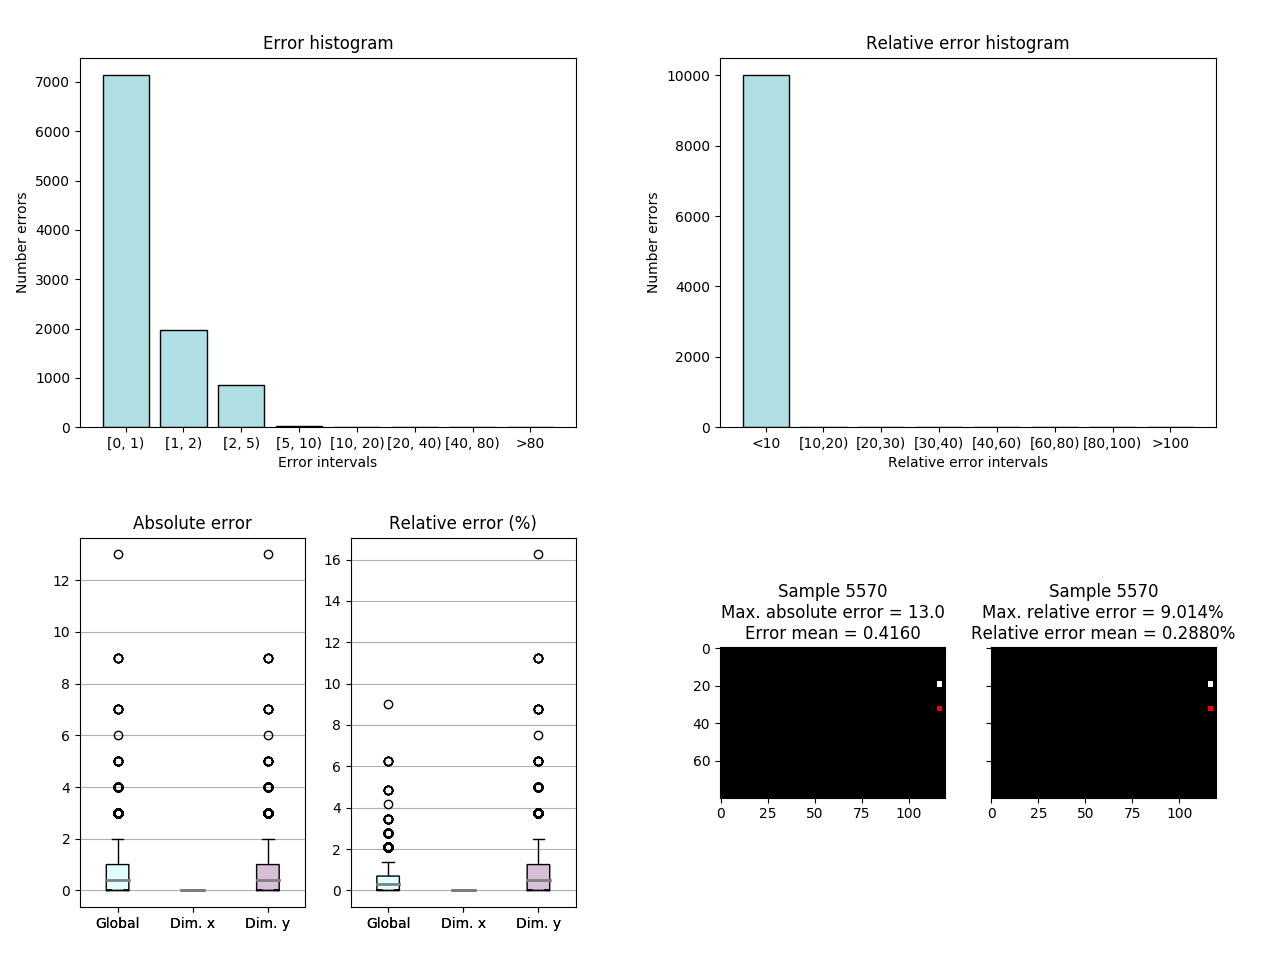
\includegraphics[width=0.8\textwidth]{ figures/test_raw/REC/ConvLSTM_simple/linear_var_100000.png}
			\caption{Resultados de ConvLSTM-1 con dinámica lineal de 2 \acrshort{dof}~(10000 muestras de \textit{test}).}
			\label{fig.raw_convlstm1_lin_var_100000}
		\end{center}
\end{figure}
\vspace{-10pt}

Al comparar los resultados con los de la red convolucional, representados en la Figura~\ref{fig.raw_norec_lin_var_100000}, se observa una gran mejoría de la estructura recurrente~(ConvLSTM-1) respecto a la no recurrente~(\acrshort{cnn}). Se reducen los valores de error relativo tanto en media como en máximo, y la cantidad de \textit{outliers} es también menor. Este hecho refuerza la conclusión extraída con las imágenes modeladas de que la recurrencia, bien aplicada, mejora las prestaciones de las redes como predictores visuales.

\subsection{Predicción con dinámicas parabólicas}
En el caso de imágenes cuyo píxel activo sigue una la dinámica parabólica, se emplea un conjunto con 100000 ejemplos, de los que 80000 se emplearán para entrenar, 10000 para validar y otros 10000 para evaluar. En la Tabla~\ref{tab.cnn_convlstm_parab} se muestra la comparación del error relativo obtenido, tanto máximo como medio, con la red sin recurrencia, la \acrshort{cnn}, y con la red recurrente \textit{ConvLSTM-1}. En dicha tabla se reafirma el hecho de que introducir de manera adecuada la recurrencia en la estructura de la red conduce a una mejora en las prestaciones.

\begin{table}[H]
	\centering
	\begin{tabular}{{l|c|c|c|c|}}
		\cline{2-5}
		& \multicolumn{2}{|c|}{\textbf{\acrshort{cnn}}} & \multicolumn{2}{|c|}{\textbf{ConvLSTM-1}} \\
		\hline
		\multicolumn{1}{|l|}{\textbf{\acrshort{dof}}} & \textbf{\textit{Max.}} & \textbf{\textit{Mean}} & \textbf{\textit{Max.}} & \textbf{\textit{Mean}}\\
		\hline 
		\multicolumn{1}{|l|}{\textbf{1~(\textit{a})}} &  0.7\% &  0.01\% & 0.7\% & 0.01\%\\ \hline
		\multicolumn{1}{|l|}{\textbf{2~(\textit{c})}} &  8.3\% &  0.07\% & 4.9\% & 0.03\%\\ \hline
		\multicolumn{1}{|l|}{\textbf{3~(\textit{b})}} &  54.7\% &  4.4\% & 22.9\% & 3.8\%\\ \hline
	\end{tabular}
	\caption{Error relativo en la dinámica parabólica con \acrshort{cnn} y ConvLSTM-1 (10000 muestras de \textit{test}).}
	\label{tab.cnn_convlstm_parab}
\end{table}
A pesar de haber mejorado los resultados obtenidos, en el caso más complejo de la dinámica, 3~\acrshort{dof}, se continúa sin conseguir una buena capacidad predictiva, lo que deja un margen de mejora a estudiar por distintas vías.

\subsection{Predicción con dinámicas sinusoidales}
Para la dinámica sinusoidal se emplea para cada caso un conjunto de 100000 muestras, que se reparten en 80000 para entrenamiento, 10000 para validación y 10000 para \textit{test}. La Tabla~\ref{tab.cnn_convlstm_sin} refleja la misma comparación que en el caso parabólico. Los resultados muestran que, a pesar del aporte de la recurrencia en las prestaciones, la mejora obtenida es muy pequeña y se continúa sin ser capaz de predecir en los casos más complejos de la dinámica sinusoidal.

\begin{table}[H]
	\centering
	\begin{tabular}{{l|c|c|c|c|}}
		\cline{2-5}
	    &\multicolumn{2}{|c|}{\textbf{\acrshort{cnn}}}
	    &\multicolumn{2}{|c|}{\textbf{ConvLSTM-1}} \\
		\hline
		\multicolumn{1}{|l|}{\textbf{\acrshort{dof}}} & \textbf{\textit{Max.}} & \textbf{\textit{Mean}} & \textbf{\textit{Max.}} & \textbf{\textit{Mean}}\\
		\hline 
		\multicolumn{1}{|l|}{\textbf{1~(\textit{f})}} & 0.7\% & 0.01\% & 0.7\% & 0.01\%\\ \hline
		\multicolumn{1}{|l|}{\textbf{2~(\textit{y0})}} & 64.0\% & 1.1\% & 44.3\% & 1.1\%\\ \hline
		\multicolumn{1}{|l|}{\textbf{3~(\textit{A})}} & $\times$ & $\times$ & 46.5\% & 3.4\%\\ \hline
		\multicolumn{1}{|l|}{\textbf{3~(\textit{c})}} & $\times$ & $\times$ & 54.1\% & 13\%\\ \hline
	\end{tabular}
	\caption{Error relativo en la dinámica sinusoidal con ConvLSTM-1 (10000 muestras de \textit{test}).}
	\label{tab.cnn_convlstm_sin}
\end{table}

\subsection{Resumen de resultados}
La Tabla~\ref{tab.convlstm1} presenta un resumen de los mejores resultados obtenidos utilizando la red \textit{ConvLSTM-1} para cada una de las dinámicas.

\begin{table}[H]
	\centering
	\begin{tabular}{{|l|c|c|}}
		\hline
		\multicolumn{2}{|c|}{\textbf{Dinámica}} & \textbf{ConvLSTM-1}\\ \hline 
		\multirow{2}{*}{Lineal}
		&1~\acrshort{dof} & \cellcolor{darkgreen}0.06\%\\
		\cline{2-3}
        &2~\acrshort{dof} & \cellcolor{darkgreen}0.29\%\\ 
        \hline
        \multirow{3}{*}{Parabólica}
        &1~\acrshort{dof} & \cellcolor{darkgreen}0.01\%\\
        \cline{2-3}
        &2~\acrshort{dof} & \cellcolor{darkgreen}0.03\%\\
        \cline{2-3}
        &3~\acrshort{dof} & \cellcolor{red}3.76\%\\ 
        \hline
        \multirow{4}{*}{Sinusoidal}
        &1~\acrshort{dof} & \cellcolor{darkgreen}0.01\%\\
        \cline{2-3}
        &2~\acrshort{dof} & \cellcolor{myorange}1.12\%\\
        \cline{2-3}
        &3~\acrshort{dof} & \cellcolor{red}3.44\%\\
        \cline{2-3}
        &4~\acrshort{dof} & \cellcolor{red}13.00\%\\ 
        \hline
	\end{tabular}
	\caption{Promedio del error relativo en \textit{test} al evaluar la red ConvLSTM-1 con imágenes modeladas y distintas dinámicas (10000 muestras de \textit{test}).}
	\label{tab.convlstm1}
\end{table}

Al igual que en el primer caso, se ha reevaluado la dinámica lineal de 1~\acrshort{dof} con 10000 muestras para que la comparación entre las redes sea equitativa.

\section{Arquitectura recurrente: ConvLSTM-4}
Para tratar de obtener una arquitectura capaz de predecir en todas las dinámicas en su caso más complejo se realizan una serie de experimentos que dan lugar a la estructura de red recurrente definida en la Figura~\ref{fig.convLSTM4}.
\vspace{10pt}
\begin{figure}[H]
		\begin{center}
			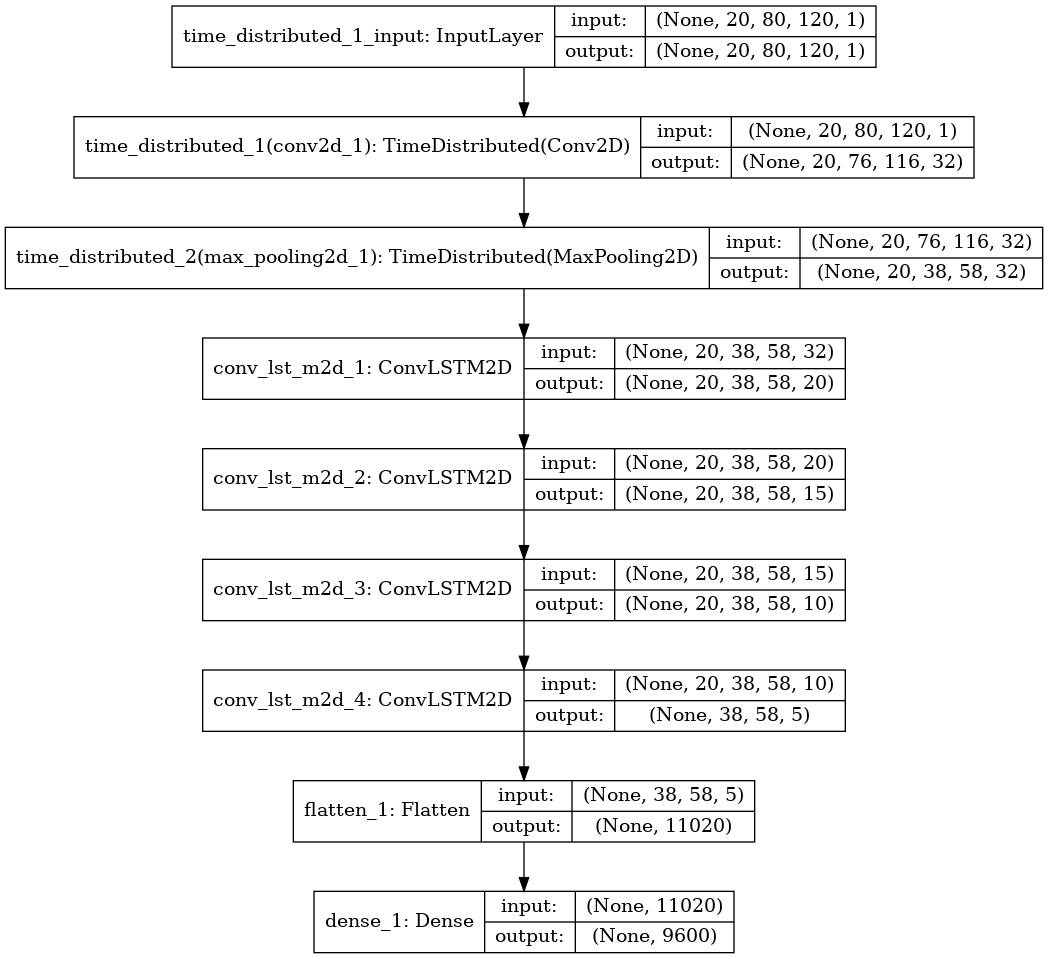
\includegraphics[width=1\textwidth]{ figures/net/REC_convLSTM_complex.png}
			\caption{Estructura de ConvLSTM-4 para imágenes crudas.}
			\label{fig.convLSTM4}
		\end{center}
\end{figure}

La nueva arquitectura se compone de 4 capas \textit{ConvLSTM} de 20, 15, 10 y 5 neuronas que vienen precedidas de una única estructura convolucional~(capa convolucional y de \textit{pooling}) para la reducción de la cantidad de valores de entrada a la red.\\

Con el objetivo de mejorar los resultados, por un lado se reduce el número de capas convolucionales previas a la recurrencia, para evitar perder demasiadas correlaciones y perjudicar a la predicción. Por otro lado, y conforme a las conclusiones extraídas de las imágenes modeladas, se opta por aumentar el número de capas \textit{ConvLSTM} que se introducen en la estructura.

\subsection{Aumento de capas}
En línea con el estudio del Apartado~\ref{ap.capas_mod}, se explora dónde situar el límite de número de capas a añadir a la estructura para obtener las mejores prestaciones. Para ello se ha utilizado el conjunto que sigue una dinámica sinusoidal de máxima complejidad, 4~\acrshort{dof}, con un total de 100000 muestras: 80000 de entrenamiento, 10000 de validación y 10000 de \textit{test}. En la Figura~\ref{fig.capas_raw} se muestra el resultado de este estudio con la evolución del error relativo según el número de capas utilizado.
\begin{figure}[H]
		\begin{center}
			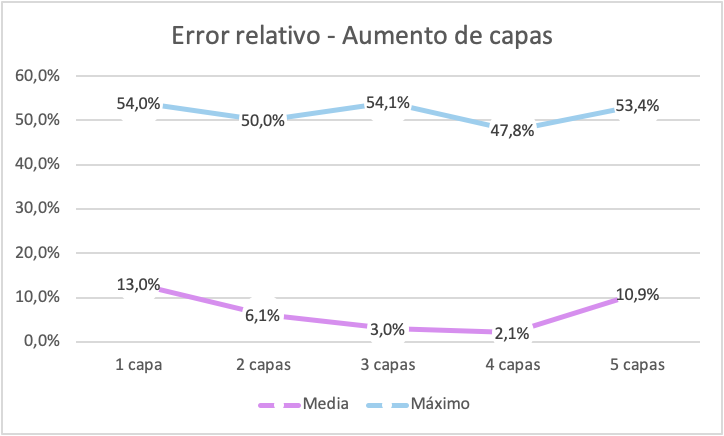
\includegraphics[width=0.7\textwidth]{ figures/test_raw/REC/ConvLSTM_complex/capas_raw.png}
			\caption{Comparación del error relativo al aumentar el número de capas ConvLSTM~(Sinusoidal, 4~\acrshort{dof}, 10000 muestras de \textit{test}).}
			\label{fig.capas_raw}
		\end{center}
\end{figure}
\vspace{-10pt}

El gráfico ilustra que a medida que se aumenta el número de capas \textit{ConvLSTM} en la estructura, las prestaciones de la misma mejoran en promedio. Sin embargo, al llegar a 4 capas se obtiene el mínimo en el valor de la media del error relativo, pues al pasar a 5 capas los resultados vuelven a empeorar. Este hecho hace que la estructura escogida esté formada por 4 capas \textit{ConvLSTM}, pues es la que mejores prestaciones ofrece.

\subsection{Predicción con dinámicas lineales}
En la Figura~\ref{fig.raw_convlstm4_lin_var_100000} se muestran los resultados obtenidos utilizando un conjunto que sigue la dinámica lineal de un \acrshort{dof}. Este conjunto consta de 100000 muestras en total, de las que 80000 se usan para el entrenamiento, 10000 para la validación y 10000 para la evaluación.

\begin{figure}[H]
		\begin{center}
			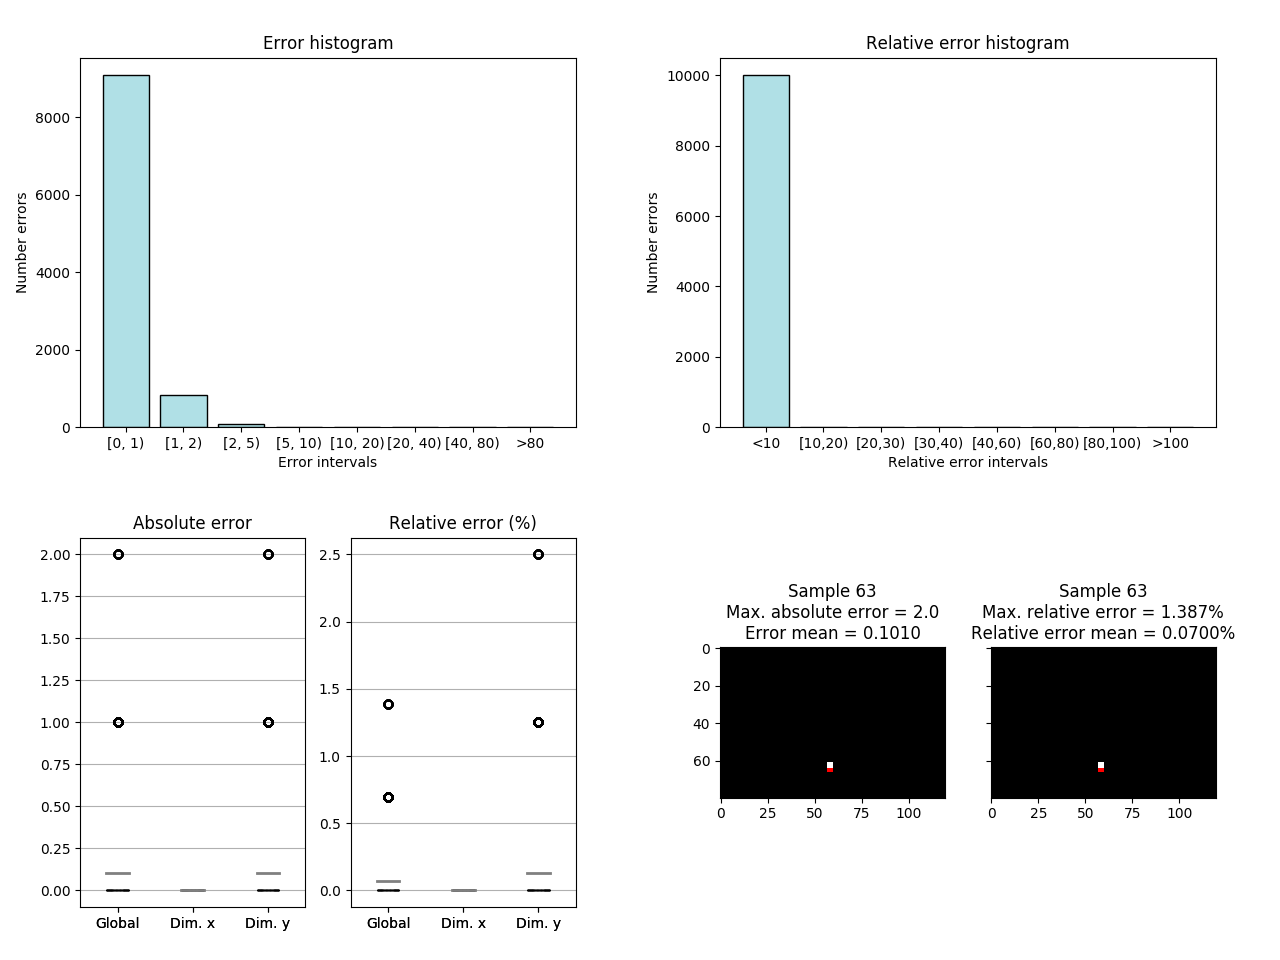
\includegraphics[width=0.8\textwidth]{ figures/test_raw/REC/ConvLSTM_complex/lin_var_100000.png}
			\caption{Resultados de ConvLSTM-4 con dinámica lineal de 1 \acrshort{dof}~(10000 muestras de \textit{test}).}
			\label{fig.raw_convlstm4_lin_var_100000}
		\end{center}
\end{figure}
\vspace{-10pt}

El aumento de número de capas tiene un claro efecto positivo en el caso más complejo de esta dinámica, reduciendo  considerablemente el error cometido y el número de \textit{outliers}.

\subsection{Predicción con dinámicas parabólicas}
Para la dinámica parabólica se emplea el mismo conjunto utilizado con la estructura de una capa, manteniendo todos los grados de libertad. En la Figura~\ref{fig.raw_convlstm4_par_var1_100000} se muestran los resultados obtenidos para este caso. Se puede comprobar que, aunque sí  hay una mejora en cuanto al valor del promedio del error relativo, se produce una mayor dispersión en los resultados que reduce la capacidad predictiva de la red.

\begin{figure}[H]
		\begin{center}
			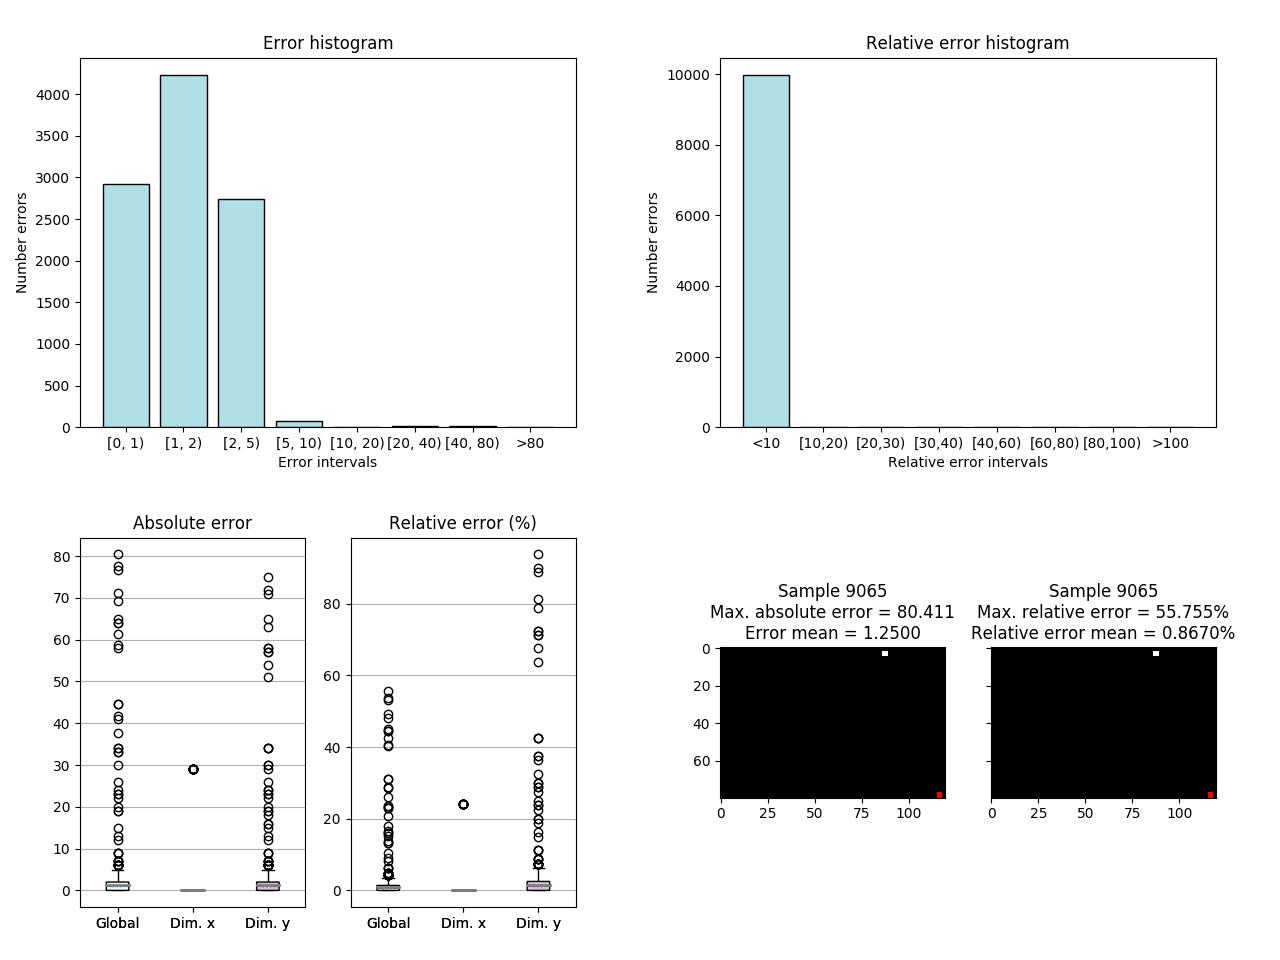
\includegraphics[width=0.8\textwidth]{ figures/test_raw/REC/ConvLSTM_complex/parabolic_var1_100000.png}
			\caption{Resultados de ConvLSTM-4 con dinámica parabólica de 2 \acrshort{dof}~(10000 muestras de \textit{test}).}
			\label{fig.raw_convlstm4_par_var1_100000}
		\end{center}
\end{figure}
\vspace{-10pt}

\subsection{Predicción con dinámicas sinusoidales}
En la última dinámica propuesta, la sinusoidal, con las redes anteriores no se conseguía predecir bien con varios \acrshort{dof}. Por este motivo la nueva estructura de red se aplica, no solo al caso más complejo de 4~\acrshort{dof}, sino también a los casos de 2 y 3 \acrshort{dof} cuyos resultados no fueron satisfactorios.\\

En la Figura~\ref{fig.raw_convlstm4_sin_var_100000} se muestran los resultados obtenidos para la dinámica con 2~\acrshort{dof}. Con la nueva estructura propuesta se consigue dominar esta dinámica en términos de media del error relativo, pero sigue existiendo un gran número de \textit{outliers} que reducen la capacidad de predicción de la red.

\begin{figure}[H]
		\begin{center}
			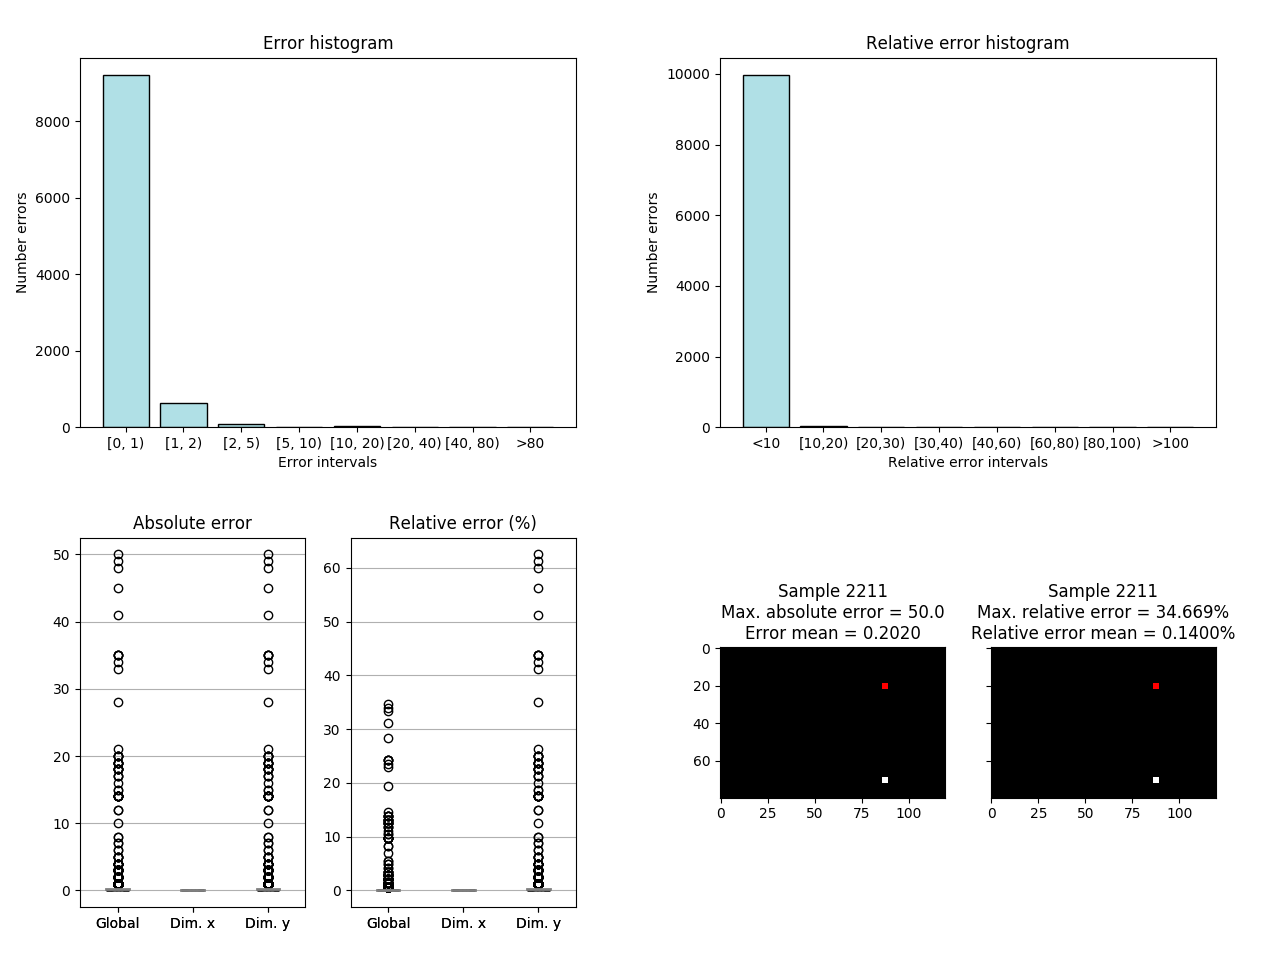
\includegraphics[width=0.8\textwidth]{ figures/test_raw/REC/ConvLSTM_complex/sin_var_100000.png}
			\caption{Resultados de ConvLSTM-4 con dinámica sinusoidal de 2 \acrshort{dof}~(10000 muestras de \textit{test}).}
			\label{fig.raw_convlstm4_sin_var_100000}
		\end{center}
\end{figure}
\vspace{-10pt}

Aumentando la complejidad con un grado de libertad más, 3 \acrshort{dof}, se obtienen los resultados mostrados en la Figura~\ref{fig.raw_convlstm4_sin_var1_100000}. La situación es muy similar al caso anterior, se mejoran los valores de promedio del error relativo, pero la presencia de múltiples \textit{outliers} hace que las prestaciones de la red se vean reducidas.\\

Para terminar con la dinámica sinusoidal, en la Figura~\ref{fig.raw_convlstm4_sin_var2_100000} se muestran los resultados obtenidos para la dinámica con 4~\acrshort{dof}. Como ocurría en el caso parabólico, a pesar de una clara mejora en los valores, la existencia de \textit{outliers} de valores elevados empeoran los resultados y perjudican a la capacidad de predicción de la red.

\begin{figure}[H]
		\begin{center}
			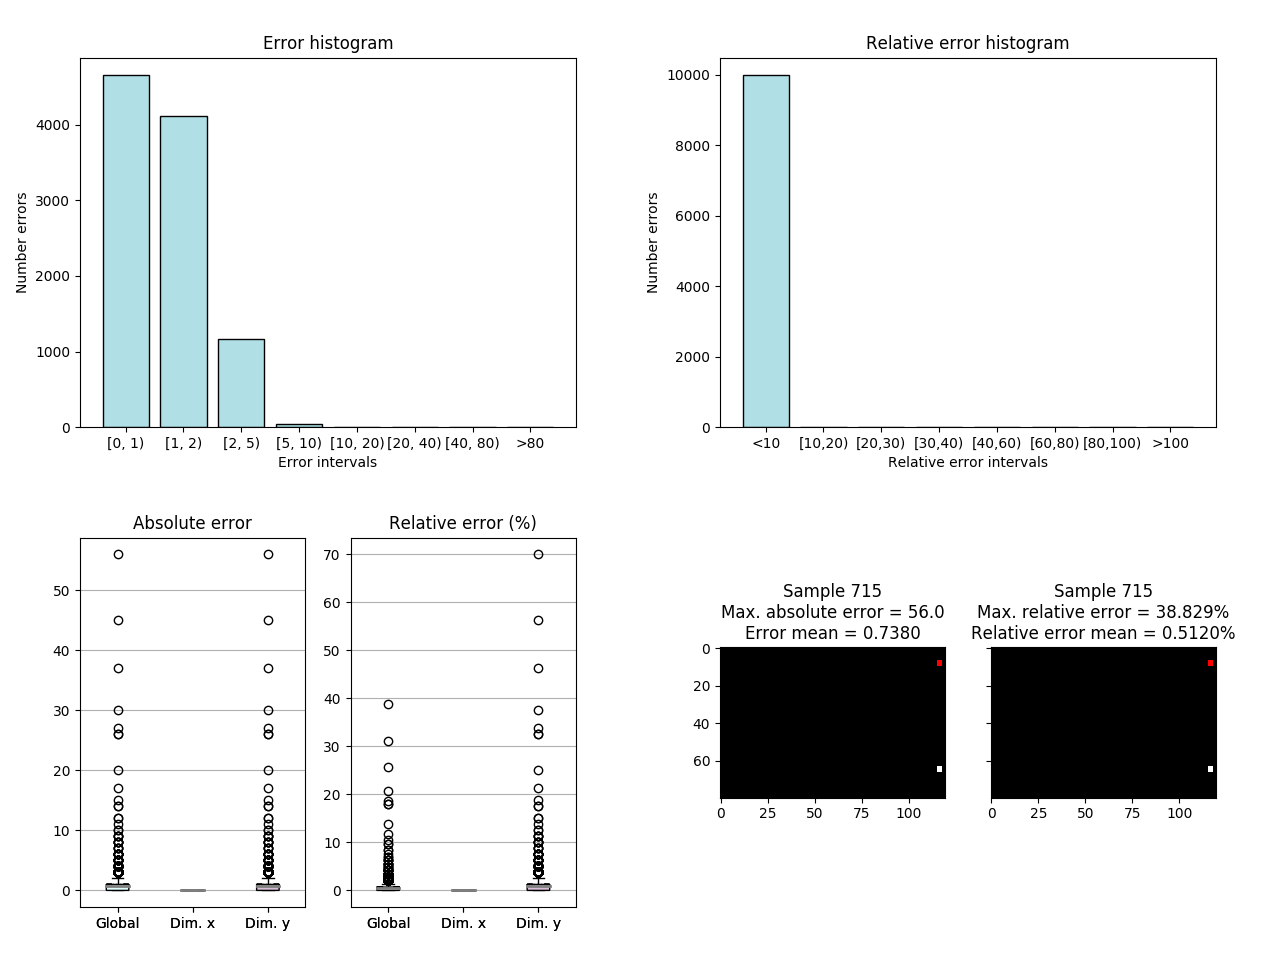
\includegraphics[width=0.8\textwidth]{ figures/test_raw/REC/ConvLSTM_complex/sin_var1_100000.png}
			\caption{Resultados de ConvLSTM-4 con dinámica sinusoidal de 3 \acrshort{dof}~(10000 muestras de \textit{test}).}
			\label{fig.raw_convlstm4_sin_var1_100000}
		\end{center}
\end{figure}
\vspace{-30pt}
\begin{figure}[H]
		\begin{center}
			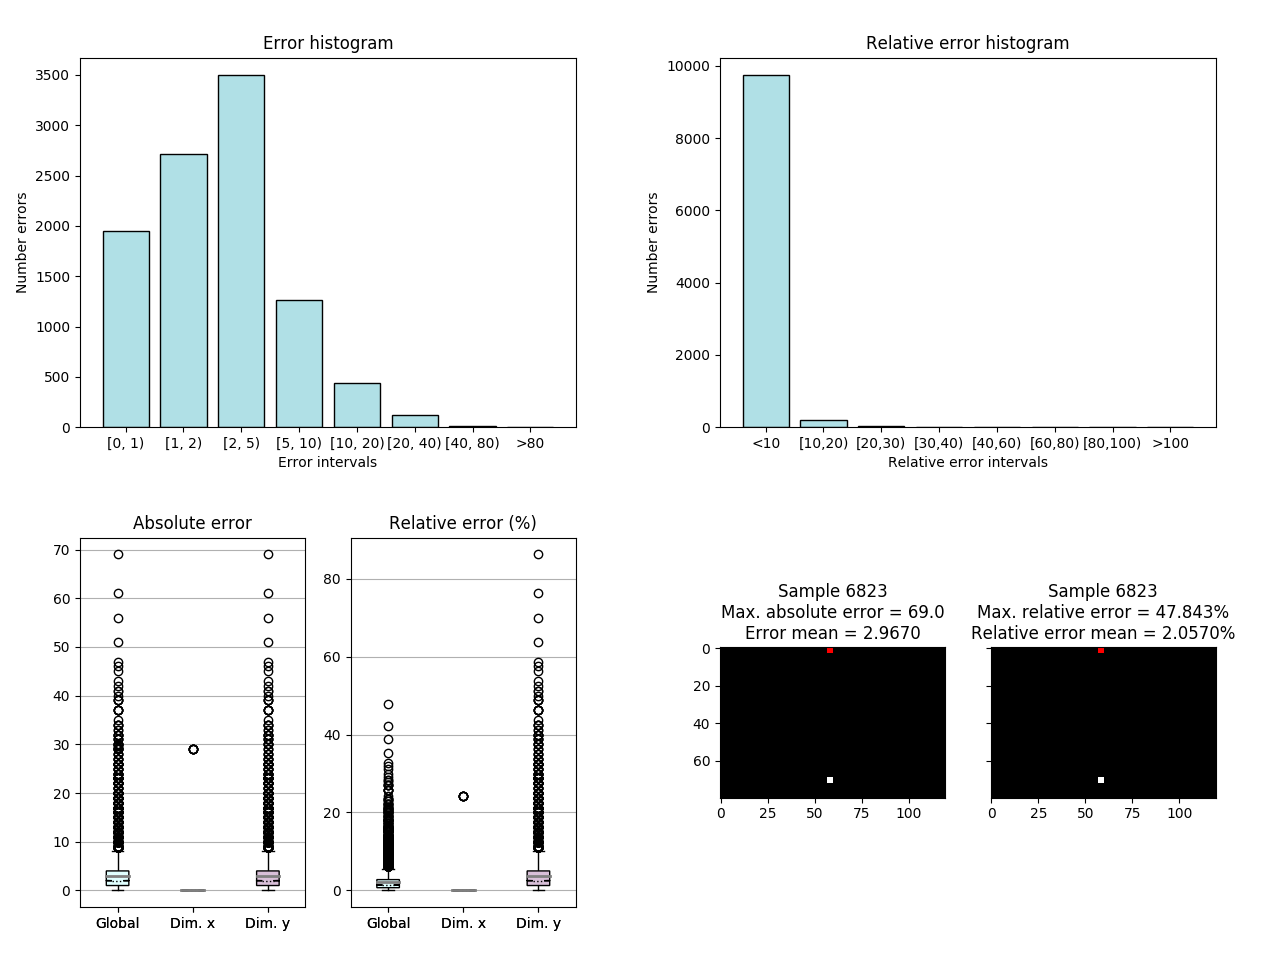
\includegraphics[width=0.8\textwidth]{ figures/test_raw/REC/ConvLSTM_complex/sin_var2_100000.png}
			\caption{Resultados de ConvLSTM-4 con dinámica sinusoidal de 4 \acrshort{dof}~(10000 muestras de \textit{test}).}
			\label{fig.raw_convlstm4_sin_var2_100000}
		\end{center}
\end{figure}
\vspace{-10pt}

\subsection{Predicción con dinámica combinada}
Por último, se realiza un experimento similar al que se realiza con imágenes modeladas, utilizando un conjunto que combine muestras de los tres tipos. Para ello se utilizan un total 33000 ejemplos que siguen una dinámica lineal, 33000 que siguen una parabólica y 34000 que siguen una sinusoidal, repartidas en una proporción de 80\%-10\%-10\% para los subconjuntos de entrenamiento, validación y \textit{test} respectivamente. Con esto, se obtienen los resultados mostrados en la Figura~\ref{fig.raw_convlstm4_mix_100000}.
\begin{figure}[H]
		\begin{center}
			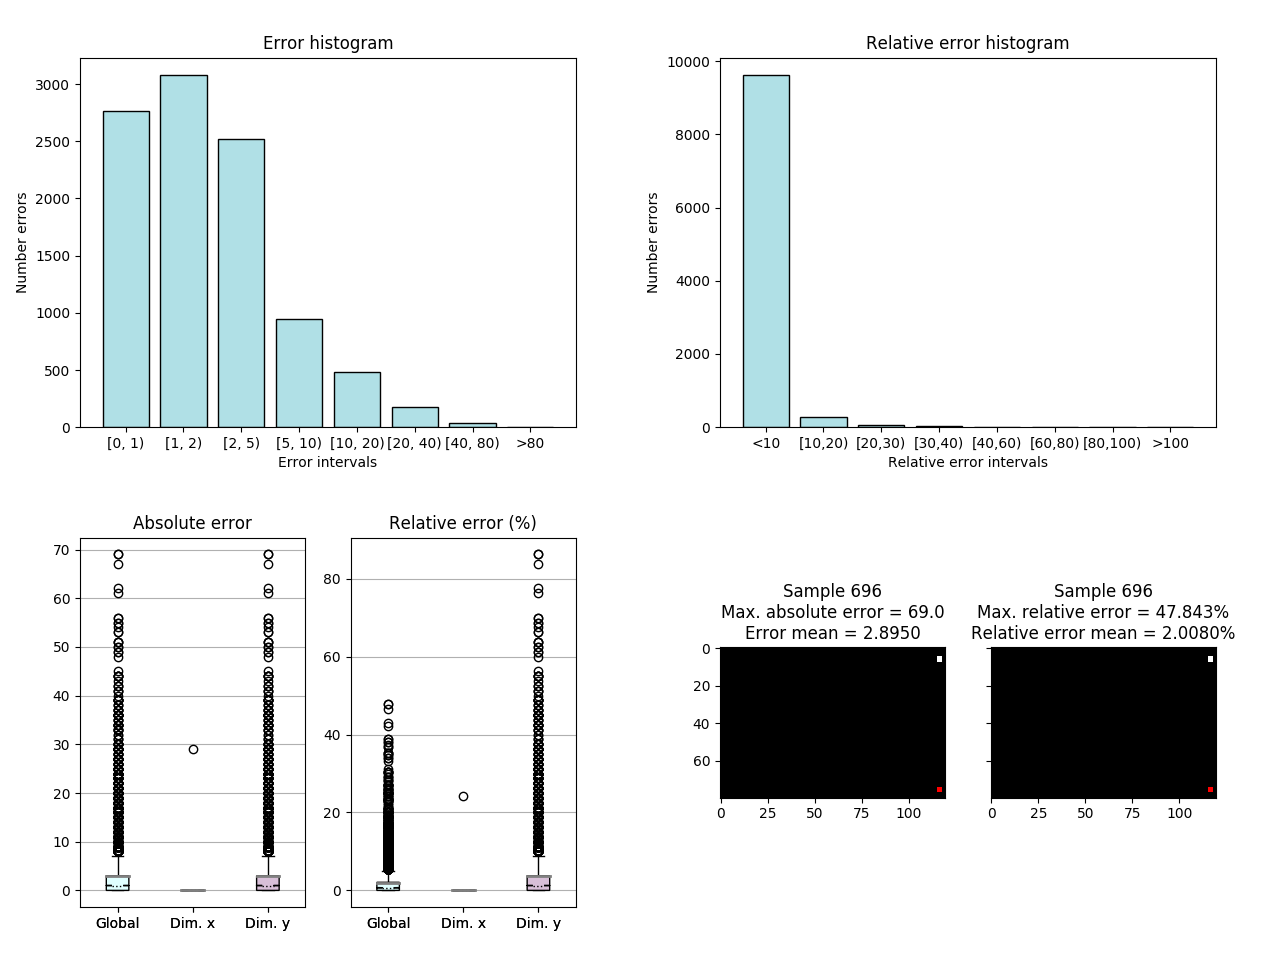
\includegraphics[width=0.8\textwidth]{ figures/test_raw/REC/ConvLSTM_complex/mix_100000.png}
			\caption{Resultados de ConvLSTM-4 con dinámica combinada~(10000 muestras de \textit{test}).}
			\label{fig.raw_convlstm4_mix_100000}
		\end{center}
\end{figure}
\vspace{-10pt}

Los resultados obtenidos son muy similares a los que se consiguen con la dinámica más compleja de todas, la sinusoidal con 4~\acrshort{dof}. Sin embargo, se obtiene una ligera mejora en el la media del error relativo está propiciada por las buenas prestaciones en el caso lineal.


\subsection{Resumen de resultados}
En la Tabla~\ref{tab.convlstm4} se muestra el resumen de los resultados obtenidos con la red \textit{LSTM-4} para las  dinámicas consideradas.
\begin{table}[H]
	\centering
	\begin{tabular}{{|l|c|c|}}
		\hline
		\multicolumn{2}{|c|}{\textbf{Dinámica}} & \textbf{LSTM-4}\\ \hline 
		\multicolumn{1}{|c|}{Lineal}
        &2~\acrshort{dof} & \cellcolor{darkgreen}0.07\%\\ 
        \hline
        \multicolumn{1}{|c|}{Parabólica}
        &3~\acrshort{dof} & \cellcolor{myorange}0.87\%\\ 
        \hline
        \multirow{3}{*}{Sinusoidal}
        &2~\acrshort{dof} & \cellcolor{greenyellow}0.14\%\\
        \cline{2-3}
        &3~\acrshort{dof} & \cellcolor{greenyellow}0.51\%\\
        \cline{2-3}
        &4~\acrshort{dof} & \cellcolor{myorange}2.06\%\\
        \hline
        \multicolumn{2}{|c|}{Combinada} & \cellcolor{myorange}2.01\%\\ \hline 
	\end{tabular}
	\caption{Promedio del error relativo en \textit{test} al evaluar la red ConvLSTM-4 con imágenes modeladas y distintas dinámicas (10000 muestras de \textit{test}).}
	\label{tab.convlstm4}
\end{table}

Como en los casos anteriores, con el objetivo de que la comparación de los resultados sea equitativa, se ha reevaluado la dinámica lineal de 1~\acrshort{dof} con 10000 muestras.\\

La estructura ConvLSTM-4 consigue mejorar los resultados en cuanto al promedio del error relativo en todos los casos, sin embargo no se consigue solucionar el problema de los \textit{outliers}. Este hecho hace que, aunque se mejoren las prestaciones de la red, éstas no alcanzan unos valores suficientes  para  concluir que la red es capaz de predecir satisfactoriamente en todas las dinámicas independientemente de su complejidad.

\section{Comparativa global}
Tras realizar los experimentos con imágenes crudas se obtiene un conjunto de redes entrenadas para las distintas dinámicas. Para  comparar de una forma rápida todas ellas, se ha elaborado la Tabla~\ref{tab.comp_raw}, que sigue el mismo código de colores especificado en la Sección~\ref{sec.comp_mod}. También se han utilizado los resultados de la dinámica lineal de 1~\acrshort{dof} obtenidos con 10000 muestras para que la comparación sea equitativa.

\begin{table}[H]
	\centering
	\begin{tabular}{{|l|c|c|c|c|}}
		\hline
		\multicolumn{2}{|c|}{\textbf{Dinámica}} & \textbf{\acrshort{cnn}} & \textbf{ConvLSTM-1} & \textbf{ConvLSTM-4}\\ \hline 
		\multirow{2}{*}{Lineal}
		&1~\acrshort{dof} & \cellcolor{darkgreen}0.07\% & \cellcolor{darkgreen}0.06\% & \cellcolor{gray!30}\\
		\cline{2-5}
        &2~\acrshort{dof} & \cellcolor{greenyellow}0.39\% & \cellcolor{darkgreen}0.29\% & \cellcolor{darkgreen}0.07\% \\ 
        \hline
        \multirow{3}{*}{Parabólica}
        &1~\acrshort{dof} & \cellcolor{darkgreen}0.01\% & \cellcolor{darkgreen}0.01\% & \cellcolor{gray!30}\\
		\cline{2-5}
        &2~\acrshort{dof} & \cellcolor{darkgreen}0.07\% & \cellcolor{darkgreen}0.03\% & \cellcolor{gray!30}\\
        \cline{2-5}
        &3~\acrshort{dof} & \cellcolor{red}4.4\%& \cellcolor{red}3.76\%& \cellcolor{myorange}0.87\%\\ 
        \hline
        \multirow{4}{*}{Sinusoidal}
        &1~\acrshort{dof} & \cellcolor{darkgreen}0.003\% & \cellcolor{darkgreen}0.01\% & \cellcolor{gray!30} \\
        \cline{2-5}
        &2~\acrshort{dof} & \cellcolor{myorange}1.12\% & \cellcolor{myorange}1.08\% & \cellcolor{greenyellow} 0.14\%\\
        \cline{2-5}
        &3~\acrshort{dof} & \cellcolor{gray!30} & \cellcolor{red}3.44\% & \cellcolor{greenyellow} 0.54\%\\
        \cline{2-5}
        &4~\acrshort{dof} & \cellcolor{gray!30} & \cellcolor{red} 13\%& \cellcolor{myorange}2.06\%\\ 
        \hline
        \multicolumn{2}{|c|}{Combinada} & \cellcolor{gray!30} & \cellcolor{gray!30} & \cellcolor{myorange}2.01\%\\ \hline 
	\end{tabular}
	\caption{Comparativa del promedio de error relativo en las distintas redes para imágenes crudas con las distintas dinámicas (10000 muestras de \textit{test}).}
	\label{tab.comp_raw}
\end{table}

Los resultados obtenidos reflejan la complejidad de la tarea de predicción con las imágenes en crudo, debido al elevado número de parámetros a encontrar.
La red que obtiene mejores resultados es la que incorpora un mayor número de capas y, además, utiliza recurrencia. Sin embargo, no se consigue dominar todas las dinámicas en su grado más complejo, con el máximo número de \acrshort{dof}. Únicamente la dinámica lineal produce unos resultados que indican que la red es capaz de predecir bien.\\

En cuanto al número de muestras utilizadas en el entrenamiento, su aumento puede aportar una mejora a las prestaciones siempre y cuando no se sobrepase un límite. Este límite viene determinado por la naturaleza de las imágenes a predecir. Si se establece un número muy elevado de muestras en el aprendizaje, se aumenta la complejidad del entrenamiento sin obtener un beneficio del mismo. Algo parecido pasa con el número de capas, incrementar en exceso este valor puede proporcionar una estructura excesivamente compleja que no solo no mejore los resultados, sino que pueda llega a empeorarlos.\\

Por otro lado, el uso de capas que analicen las relaciones espaciales junto con las temporales (\textit{ConvLSTM}) introduce una mejora en las prestaciones de la red. Sin embargo, si se separan ambos tipos de relación (\acrshort{cnn}+\acrshort{lstm}), no solo no se obtienen mejores resultados que sin recurrencia, se reduce por completo la capacidad predictiva de la red. Además, el número de capas utilizado repercute en los resultados, introduciendo una mejora en los resultados de promedio del error relativo a medida que se aumentan, hasta 4 capas, pero sin solucionar el problema de los \textit{outliers} que empeora la predicción.\\

Con todo lo expuesto anteriormente se concluye que, con imágenes crudas, ConvLSTM-4 es  la red que mejores resultados obtiene. Esta red consigue dominar por completo únicamente la dinámica lineal. Para el resto de dinámicas se deja la puerta abierta a nuevas investigaciones que permitan reducir el número de valores atípicos y mejorar las prestaciones para los casos más complejos.